\documentclass[11pt,a4paper]{report}

%%%%%%%%%%%%%%%%%%%%%%%%%%%%%%%%%%%%
% PACKAGES
%%%%%%%%%%%%%%%%%%%%%%%%%%%%%%%%%%%%
\usepackage[T1]{fontenc}
\usepackage[utf8]{inputenc}
\usepackage{amsmath,amssymb}
\usepackage{siunitx}
\usepackage{graphicx}
\usepackage[hidelinks,hypertexnames=false]{hyperref}
\usepackage{geometry}
\usepackage{setspace}
\usepackage{booktabs}
\usepackage{multirow}
\usepackage{array}
\usepackage{tikz}
\usepackage{cite}
\geometry{margin=1in}

\usetikzlibrary{positioning, fit, backgrounds, arrows,arrows.meta}

% Optional: if you want [H] placement
\usepackage{float}
\geometry{margin=1in}
\onehalfspacing

%%%%%%%%%%%%%%%%%%%%%%%%%%%%%%%%%%%%
% DOCUMENT
%%%%%%%%%%%%%%%%%%%%%%%%%%%%%%%%%%%%
\begin{document}

\chapter{Artificial Intelligence in Gas Dynamics}


\section{Introduction}
Gas dynamics, the study of compressible fluid flows, is foundational to aerospace, mechanical, and chemical engineering \cite{White2011}. Traditional approaches rely on analytical solutions, empirical correlations, and numerical solvers of the governing partial differential equations. Canonical one-dimensional problems---Fanno flow, Rayleigh flow, shock tubes, and nozzle expansions---admit exact or semi-analytical solutions under idealized assumptions and serve as benchmarks for both teaching and code verification \cite{Anderson1990, Pontes2019, Anderson2021}.

Although these methods are accurate within their domain of validity, they encounter limitations in more demanding settings:
\begin{itemize}
    \item \textbf{Computational cost.} Iterative solvers become expensive when many evaluations are required, as in parametric design studies, optimization loops, or real-time applications.
    \item \textbf{Limited flexibility.} Closed-form correlations rely on idealizations such as constant properties or constant friction factors, which restrict their applicability to realistic geometries.
    \item \textbf{Inverse problems.} Recovering unknown parameters from sparse or noisy measurements typically requires bespoke optimization procedures and ad-hoc regularization.
\end{itemize}

Artificial intelligence (AI) techniques, in particular neural networks and physics-informed neural networks (PINNs), provide complementary tools that can mitigate each of these limitations \cite{Raissi2019PINN, Michaloglou2025, Ren2025, Roohi2025}. AI is not a substitute for classical theory: the goal is not to rediscover known solutions, but rather to emulate, accelerate, and augment traditional analysis while remaining physically consistent. To make this concrete, the present chapter adopts the \textbf{Fanno flow problem} as a representative, well-controlled test case.

\subsection{Motivation for AI in Gas Dynamics}

Two distinct mechanisms make AI useful in gas dynamics. First, neural network \emph{surrogates} learn the input--output mapping of an existing model and replace it with a fast, differentiable approximation; once trained, evaluation is essentially the cost of a forward pass. Second, \emph{physics-informed neural networks} embed the governing equations directly into the training objective, so that the learned solution satisfies conservation laws by construction even when training data are sparse or noisy \cite{Raissi2019PINN, Michaloglou2025}. The two mechanisms can also be combined.

These capabilities translate into concrete benefits for engineering practice:

\begin{itemize}
    \item \textbf{Efficient approximation.} Neural surrogates approximate complex solution manifolds with orders-of-magnitude speedups relative to repeated numerical solves, enabling parametric studies, optimization, and real-time prediction \cite{Ren2025}.
    \item \textbf{Sparse and noisy data.} Physics-informed frameworks integrate physical constraints with limited observations, allowing accurate reconstruction of flow fields where experiments are incomplete or contaminated \cite{Michaloglou2025}.
    \item \textbf{Inverse problems.} PINNs have been used to identify friction factors, heat-source distributions, and boundary inputs from indirect measurements while still enforcing the governing equations \cite{Raissi2019PINN, Michaloglou2025, Roohi2025}.
    \item \textbf{Design-space exploration.} Once trained, surrogates make it tractable to sweep over geometries, boundary conditions, or operating regimes that would be prohibitive with classical solvers alone \cite{Ren2025}.
\end{itemize}

These benefits come with non-trivial training challenges. The composite loss functions used in PINNs---PDE/ODE residuals, boundary conditions, and (optional) observational data---produce non-convex optimization landscapes whose minima are sensitive to loss weights, network architecture, and collocation-point distribution \cite{Urban2025, Lu2021hPINN}. PINNs can also struggle to capture sharp gradients or discontinuities without targeted strategies such as adaptive sampling, loss re-weighting, or domain decomposition \cite{Urban2025, Ren2025, Kharazmi2021}. Active research addresses these issues with adaptive weighting, collocation refinement, and hybrid training schemes \cite{Jagtap2020, Cuomo2022, Ren2025}.


\subsection{Applications of AI in Gas Dynamics}

Classical gas dynamics problems---such as Fanno flow, Rayleigh flow, oblique shocks and expansions, nozzle flows, and shock tube problems---are traditionally addressed using analytical or semi-analytical methods derived from conservation laws and simplifying assumptions. While these approaches provide exact or closed-form solutions under idealized conditions \cite{Anderson1990,Pontes2019,Anderson2021}, they can become computationally expensive, inflexible, or impractical in more complex scenarios \cite{White2011,Duraisamy2019}.

AI-based models, particularly neural network surrogates and physics-informed neural networks (PINNs), can complement classical theory by enabling rapid evaluation, inverse problem solving, and design space exploration \cite{Raissi2019PINN,Roohi2025,Michaloglou2025,Ren2025}. Building on the general PINN capabilities discussed earlier, the following examples illustrate how AI is applied to canonical gas dynamics problems:


\begin{itemize}
    \item \textbf{Fanno Flow:} AI models, particularly physics-informed neural networks (PINNs), can learn the nonlinear relationship between duct friction, Mach number, and thermodynamic properties along a constant-area duct. Once trained, such models enable rapid prediction of the complete flow field for varying friction factors or inlet Mach numbers.
    
    \item \textbf{Rayleigh Flow:} In flows with heat addition or extraction, AI can efficiently capture the coupling between thermal energy input and flow acceleration or deceleration. PINNs can enforce the governing energy equation and associated thermodynamic constraints, producing physically consistent solutions even when only limited temperature or pressure data are available.
    
    \item \textbf{Oblique Shock and Expansion Waves (Theta--Beta--Mach Relation):} Neural networks can approximate the highly nonlinear trigonometric relationships governing oblique shocks and Prandtl--Meyer expansion fans. After training, AI models provide near-instantaneous evaluation of shock angles, downstream Mach numbers, and pressure ratios over broad ranges of upstream Mach number and flow deflection angle.
    
    \item \textbf{Nozzle Flows:} AI can learn the mapping between nozzle geometry, inlet conditions, and exit flow properties, enabling rapid evaluation of multiple design configurations or operating regimes. Physics-informed approaches can embed the quasi-one-dimensional governing equations to ensure conservation of mass, momentum, and energy throughout the nozzle.
    
    \item \textbf{Burgers' Equation:} As the canonical scalar nonlinear conservation law, Burgers' equation captures the convection--diffusion competition that drives shock formation in compressible flows. Although it is a simplification of the full Euler system, it retains the nonlinear advection mechanism responsible for characteristic crossing and discontinuity formation, and admits the analytical Cole--Hopf linearization in its viscous form. AI models, particularly PINNs, can recover the full space--time solution from the governing PDE alone, providing a transparent benchmark for shock-resolving learning strategies that bridges the steady Fanno problem and the full shock-tube system.
    
    \item \textbf{Shock Tube Problems:} AI models can emulate the time-dependent propagation of shock and expansion waves in shock tubes, producing fast approximations of pressure, density, and velocity fields. Inverse learning techniques may also be used to infer initial conditions---such as driver pressure or diaphragm location---from sparse downstream measurements.
\end{itemize}

To maintain clarity, rigor, and depth, this chapter develops two complementary canonical demonstrators that anchor the chapter to the wider theme of shock-wave dynamics. The \textbf{Fanno flow problem} provides the steady, one-dimensional ODE benchmark: it admits exact analytical solutions, exhibits strong nonlinear behavior near the sonic point, and supports a clear forward formulation from inlet conditions and friction to local flow properties. The \textbf{Burgers' equation} provides the unsteady, one-dimensional PDE benchmark: it captures the spontaneous formation of a shock from smooth initial data, admits an analytical reference through the Cole--Hopf transformation, and serves as the scalar prototype for the full Euler shock-tube system. Treating these two problems in sequence allows the effectiveness, limitations, and interpretability of AI-based approaches to be assessed against analytical references in both the steady-ODE and unsteady-PDE regimes. A complementary recent treatment using deep-learning surrogates across several canonical compressible-flow problems is given by Roohi \cite{Roohi2025}.


\section{Fanno Flow}

\subsection{Introduction and Physical Intuition}

Fanno flow describes the behavior of a compressible fluid moving through a constant-area duct in which friction is present. Unlike flow in a nozzle, where acceleration or deceleration arises from changes in cross-sectional area, in Fanno flow the velocity changes are driven solely by frictional effects at the duct walls. This classical problem in gas dynamics has practical relevance to pipelines, engine intakes, and HVAC systems, and provides insight into the limits of steady compressible flow under frictional constraints.

To build physical intuition, we begin with the fundamental conservation laws. In a steady, one-dimensional duct, the mass flow rate is constant:

\[
\dot{m} = \rho u A,
\]

where \(\rho\) is the density, \(u\) the velocity, and \(A\) the duct cross-sectional area. This implies that any change in velocity must be accompanied by a corresponding change in density. In differential form:

\[
\frac{d\rho}{\rho} + \frac{du}{u} = 0,
\]

which captures the tradeoff between density and velocity along the duct.

The momentum balance accounts for wall friction. For a small duct segment of length \(dx\), the differential momentum equation is

\[
dp + \rho u\, du + \frac{4 \tau_w}{D}\, dx \;=\; dp + \rho u\, du + \frac{2 f \rho u^{2}}{D}\, dx = 0,
\]

where \(f\) is the Fanning friction factor, \(D\) is the duct diameter, and the wall shear stress is \(\tau_w = f \rho u^{2} / 2\). The wall force per unit volume of a circular duct is \(4\tau_w/D\), which gives the friction term above and fixes the factor of four appearing in the dimensionless friction length \(4fL^{*}/D\) used throughout this chapter.

Energy conservation in adiabatic flow requires that enthalpy plus kinetic energy remain constant:

\[
dh + u\, du = 0 \quad \Rightarrow \quad c_p\, dT + u\, du = 0,
\]

where \(h\) is the enthalpy and \(c_p\) the specific heat at constant pressure. This ensures that friction reduces total pressure but the total energy of the flow remains conserved.

Introducing the Mach number \(M = u/a\), with \(a = \sqrt{\gamma R T}\) as the local speed of sound, and combining continuity, momentum, and energy equations leads to the Fanno relation:

\[
\frac{4 f L^*}{D} = \frac{1 - M^2}{\gamma M^2} + \frac{\gamma+1}{2\gamma} \ln \left[ \frac{(\gamma+1) M^2}{2 + (\gamma-1) M^2} \right],
\]

where \(L^*\) is the distance along the duct. The left-hand side is the dimensionless friction length, while the right-hand side depends solely on the Mach number. This Fanno function provides a direct mapping from friction length to Mach number along the duct.

Physically, the Fanno function reveals key characteristics:

\begin{itemize}
    \item \textbf{Subsonic inlet:} Friction decelerates the flow and increases static pressure.  
    \item \textbf{Supersonic inlet:} Friction accelerates the flow and decreases static pressure.  
    \item \textbf{Choking:} There exists a maximum duct length beyond which steady flow is impossible, occurring when \(M = 1\).
\end{itemize}

Once the local Mach number $M(x)$ is recovered from the Fanno relation, the auxiliary flow properties follow from the sonic-referenced Fanno ratios
\[
\frac{T}{T^{*}} = \frac{\gamma+1}{2 + (\gamma-1)M^{2}},
\qquad
\frac{P}{P^{*}} = \frac{1}{M}\sqrt{\frac{\gamma+1}{2 + (\gamma-1)M^{2}}},
\qquad
\frac{\rho}{\rho^{*}} = \frac{1}{M}\sqrt{\frac{2 + (\gamma-1)M^{2}}{\gamma+1}},
\]
\[
\frac{P_{0}}{P_{0}^{*}} = \frac{1}{M}\left[ \frac{2 + (\gamma-1)M^{2}}{\gamma+1} \right]^{\frac{\gamma+1}{2(\gamma-1)}},
\]
where the starred quantities denote the sonic reference state reached at the end of the duct. It is worth emphasising that these are \emph{not} isentropic relations. Fanno flow is adiabatic, so the stagnation temperature $T_{0}$ is constant along the duct, but friction generates entropy and the stagnation pressure $P_{0}$ therefore decreases monotonically towards the sonic point. This loss of stagnation pressure at constant stagnation temperature is the defining thermodynamic signature of the Fanno process, and it is the reason the static pressure cannot be obtained from the isentropic formula. This forward map from $M$ to $(T/T^{*},\, P/P^{*},\, P_{0}/P_{0}^{*},\, 4fL^{*}/D)$ is the analytical reference used throughout this chapter.

\section{Modeling the Fanno Flow Problem}

Classical gas dynamics problems, such as Fanno flow, are ideal candidates for exploring artificial intelligence (AI) approaches due to their nonlinear behavior, availability of exact analytical solutions, and a clear forward problem formulation. This section presents a systematic, step-by-step demonstration of AI methodologies for Fanno flow, starting from classical regression, moving through feedforward surrogate neural networks, and culminating with physics-informed neural networks (PINNs) for the forward Fanno map.   

The emphasis is placed on understanding how feature engineering and model choice
influence predictive performance, rather than on replacing the underlying
analytical solution.

\subsection{Data Generation and Feature Engineering}
\label{sec:feature_engineering}

Using the analytical Fanno function $\Phi(M)$ introduced earlier:

\begin{equation}
\label{eq:fanno_function}
\Phi(M) \;\equiv\; \frac{4 f L^{*}}{D} \;=\;
\frac{1 - M^{2}}{\gamma\, M^{2}} \;+\; \frac{\gamma + 1}{2\,\gamma}\,
\ln\!\left( \frac{(\gamma + 1)\,M^{2}}{2 + (\gamma - 1)\,M^{2}} \right),
\end{equation}

we generate a dense, noise-free dataset by drawing $20{,}000$ Mach numbers uniformly from $0.05 \le M \le 5.0$, deliberately spanning subsonic, transonic, and supersonic regimes. For each $M$ the corresponding Fanno function value $\Phi(M)$ is computed analytically, along with derived flow properties such as static pressure $P(M)$, density $\rho(M)$, and temperature $T(M)$ as defined in the previous subsection. The very narrow band around $M = 1$ is included in the dataset but the validation tables and error plots flag the sonic point explicitly because the relative-error metric $|\hat{y}-y|/|y|$ becomes ill-defined where $y = 4fL^{*}/D$ vanishes.  

This dataset forms the foundation for supervised learning and surrogate modeling.

To improve the ability of AI models to learn the nonlinear Fanno relation, a set of engineered features is constructed for each Mach number:

\begin{equation}
\mathbf{x} = 
\begin{bmatrix}
M, & M^2, & 1/M, & 1/M^2, & \log(M)
\end{bmatrix}^T.
\end{equation}

Each feature targets a known structural component of the Fanno function: $M$ and $M^{2}$ capture the linear and quadratic trends, $1/M$ and $1/M^{2}$ encode the reciprocal singularity at $M\to 0$, and $\ln M$ matches the logarithmic term. By embedding the analytical structure directly into the input space, the learning problem is reduced to a nearly linear one and the regression algorithm no longer has to rediscover these behaviours from data.

All features are then standardized to zero mean and unit variance,
\begin{equation}
\tilde{x}_i = \frac{x_i - \mu_i}{\sigma_i},
\end{equation}
where $\mu_i$ and $\sigma_i$ are computed from the training portion only. Table~\ref{tab:feature_examples} lists raw feature values at representative Mach numbers and Table~\ref{tab:standardized_features} lists the corresponding standardized values, showing how the heterogeneous original scales are mapped onto a common, balanced range that stabilizes optimization.

\begin{table}[h!]
\centering
\caption{Engineered features $M^2$, $1/M$, $1/M^2$, and $\ln M$ at representative Mach numbers.}
\label{tab:feature_examples}
\begin{tabular}{c c c c c}
\toprule
$M$ & $M^2$ & $1/M$ & $1/M^2$ & $\ln(M)$ \\
\midrule
0.2  & 0.04   & 5.0    & 25.0   & -1.609 \\
0.5  & 0.25   & 2.0    & 4.0    & -0.693 \\
0.8  & 0.64   & 1.25   & 1.5625 & -0.223 \\
1.0  & 1.0    & 1.0    & 1.0    & \phantom{-}0.0 \\
1.5  & 2.25   & 0.667  & 0.444  & \phantom{-}0.405 \\
2.0  & 4.0    & 0.5    & 0.25   & \phantom{-}0.693 \\
\bottomrule
\end{tabular}
\end{table}

\begin{table}[h!]
\centering
\caption{Standardized feature values $\tilde{x}_i$ corresponding to Table~\ref{tab:feature_examples}.}
\label{tab:standardized_features}
\begin{tabular}{c c c c c}
\toprule
$M$ & $\widetilde{M^2}$ & $\widetilde{1/M}$ & $\widetilde{1/M^2}$ & $\widetilde{\ln(M)}$ \\
\midrule
0.20 & $-1.126$ & $\phantom{-}2.236$  & $\phantom{-}0.863$  & $-2.556$ \\
0.50 & $-1.098$ & $\phantom{-}0.585$  & $-0.007$            & $-1.522$ \\
0.80 & $-1.046$ & $\phantom{-}0.173$  & $-0.108$            & $-0.992$ \\
1.00 & $-0.997$ & $\phantom{-}0.035$  & $-0.132$            & $-0.740$ \\
1.50 & $-0.829$ & $-0.148$            & $-0.155$            & $-0.283$ \\
2.00 & $-0.594$ & $-0.240$            & $-0.163$            & $\phantom{-}0.042$ \\
\bottomrule
\end{tabular}
\end{table}



\subsection{Classical Regression Models}
Before introducing neural networks or physics-informed approaches, it is instructive to consider classical regression. These models are simple, computationally inexpensive, and provide a transparent benchmark for more advanced AI methods. In general, regression is used to approximate an unknown function from observed input-output pairs. 

For the Fanno function, which is strongly nonlinear and exhibits a singularity near Mach one, three classical regression approaches were considered:

\begin{itemize}
    \item \textbf{Linear Regression:} Serves as a baseline to evaluate how much of the Fanno function's behavior can be captured by a simple linear approximation.  
    \item \textbf{Polynomial Regression:} Introduces higher-order terms to model the nonlinear dependence of the Fanno function on Mach number. Polynomial regression is capable of representing curvature and can approximate singular behavior if the degree is chosen appropriately.  
    \item \textbf{Ridge and Lasso Regression:} Regularized models that mitigate overfitting when polynomial terms are used. Ridge penalizes large coefficients uniformly, while Lasso promotes sparsity, which can improve generalization and numerical stability.
\end{itemize}

Although the Fanno flow relations are nonlinear in primitive variables,
the strong performance of linear regression in this study is a direct
consequence of the chosen feature representation. Since the engineered
features mirror the functional structure of the analytical solution,
the resulting mapping between inputs and outputs becomes nearly linear
over most of the Mach number range.

As a result, even simple linear models are able to capture the dominant
trends with high accuracy, while more flexible models primarily refine
local behavior near the sonic singularity.

\subsubsection{Training Procedure}

The regression task is formulated as a supervised learning problem:

\begin{equation}
\mathbf{x} = \mathcal{T}(M), \qquad y = \Phi(M),
\end{equation}

where the feature transformation $\mathcal{T}(M)$ includes:

\begin{equation}
\mathcal{T}(M) = [M, M^2, 1/M, 1/M^2, \log(M)].
\end{equation}

These features are designed to capture the linear, nonlinear, reciprocal, and logarithmic behaviors of the Fanno function. The target variables $\mathbf{y}$ correspond to the normalized Fanno flow quantities:

\begin{equation}
\mathbf{y} = [T/T^*, \, P/P^*, \, P_0/P_0^*, \, 4fL^*/D],
\end{equation}

computed using the analytical Fanno solution for each Mach number. These variables capture temperature, pressure, total pressure, and frictional effects along the duct.  

The dataset of Section~\ref{sec:feature_engineering} ($20{,}000$ samples in $M \in [0.05, 5.0]$) is randomly split into training and validation sets, with $25\%$ of the samples held out for validation. Features are standardized to zero mean and unit variance using statistics computed on the training portion only, exactly as described in Section~\ref{sec:feature_engineering} (Table~\ref{tab:standardized_features}); the same standardizer is then applied to the held-out data so that no validation information leaks into the training pipeline.

The regression model is trained by minimizing the mean squared error (MSE):

\begin{equation}
\mathcal{L}_\text{MSE} = \frac{1}{N} \sum_{j=1}^{N} \left( y_j - \hat{y}_j \right)^2,
\end{equation}

where $N$ is the number of training samples and $\hat{y}_j$ is the model prediction.


\subsubsection{Model Evaluation and Selection}
Models were evaluated on the validation set using three standard regression metrics:

\begin{itemize}
    \item \textbf{Coefficient of Determination ($R^2$):} Proportion of variance in the target explained by the model. $R^2 = 1$ indicates perfect prediction.
    \item \textbf{Mean Absolute Error (MAE):} 
    \begin{equation}
        \text{MAE} = \frac{1}{N} \sum_{i=1}^{N} \left| \hat{y}_i - y_i \right|,
    \end{equation}
    measuring the average absolute difference between predictions and true values.
    \item \textbf{Root Mean Squared Error (RMSE):} 
    \begin{equation}
        \text{RMSE} = \sqrt{\frac{1}{N} \sum_{i=1}^{N} (\hat{y}_i - y_i)^2},
    \end{equation}
    which penalizes larger errors more heavily.
\end{itemize}

Table~\ref{tab:model_comparison} summarizes model performance across the four outputs. The \textbf{third-degree Polynomial Ridge Regression} achieves the lowest errors and highest $R^2$ values, making it the selected best-performing model.

\begin{table}[htbp]
\centering
\small
\setlength{\tabcolsep}{7pt}
\renewcommand{\arraystretch}{1.12}
\caption{Performance comparison of regression models on validation data ($20{,}000$ samples, $25\%$ held out). Best-performing model highlighted in bold.}
\label{tab:model_comparison}
\begin{tabular}{@{} >{\raggedright\arraybackslash}p{2.6cm} l r r r @{}}
\toprule
\textbf{Model} & \textbf{Output} & \textbf{$R^2_\text{val}$} & \textbf{MAE$_\text{val}$} & \textbf{RMSE$_\text{val}$} \\
\midrule
\multirow{4}{=}{\raggedright Linear}
  & $T/T^*$     & 0.999504 & 0.006371 & 0.007227 \\
  & $P/P^*$     & 0.999999 & 0.001635 & 0.001985 \\
  & $P_0/P_0^*$ & 0.995287 & 0.357784 & 0.422750 \\
  & $4fL^*/D$   & 1.000000 & 0.002096 & 0.003014 \\
\addlinespace
\multirow{4}{=}{\raggedright Ridge\\[1pt]\scriptsize($\alpha=10^{-3}$)}
  & $T/T^*$     & 0.999504 & 0.006371 & 0.007227 \\
  & $P/P^*$     & 0.999999 & 0.001635 & 0.001985 \\
  & $P_0/P_0^*$ & 0.995287 & 0.357786 & 0.422750 \\
  & $4fL^*/D$   & 1.000000 & 0.002095 & 0.003014 \\
\addlinespace
\multirow{4}{=}{\raggedright\textbf{Poly-Ridge}\\[1pt]\scriptsize\textbf{(deg.\ 3)}}
  & \textbf{$T/T^*$}     & \textbf{1.000000} & \textbf{0.000042} & \textbf{0.000051} \\
  & \textbf{$P/P^*$}     & \textbf{1.000000} & \textbf{0.000009} & \textbf{0.000010} \\
  & \textbf{$P_0/P_0^*$} & \textbf{1.000000} & \textbf{0.000013} & \textbf{0.000015} \\
  & \textbf{$4fL^*/D$}   & \textbf{1.000000} & \textbf{0.000029} & \textbf{0.000033} \\
\bottomrule
\end{tabular}
\end{table}

The relative error between the predicted and analytical Fanno values is defined as:

\begin{equation}
\varepsilon_\mathrm{rel} = 100 \times \frac{|\hat{y} - y|}{y} \, (\%),
\end{equation}

where $y$ denotes the exact Fanno solution and $\hat{y}$ the prediction from the regression model. This metric highlights regions where the model deviates significantly from the analytical solution, with larger values indicating higher discrepancy. Figure~\ref{fig:poly_ridge_error} illustrates the relative error of the Polynomial Ridge Regression predictions across the Mach number range. The model achieves very low errors for all four target variables except near $M=1$, where the Fanno function is singular, demonstrating the model's strong predictive capability over both subsonic and supersonic regimes.

\begin{figure}[h!]
\centering
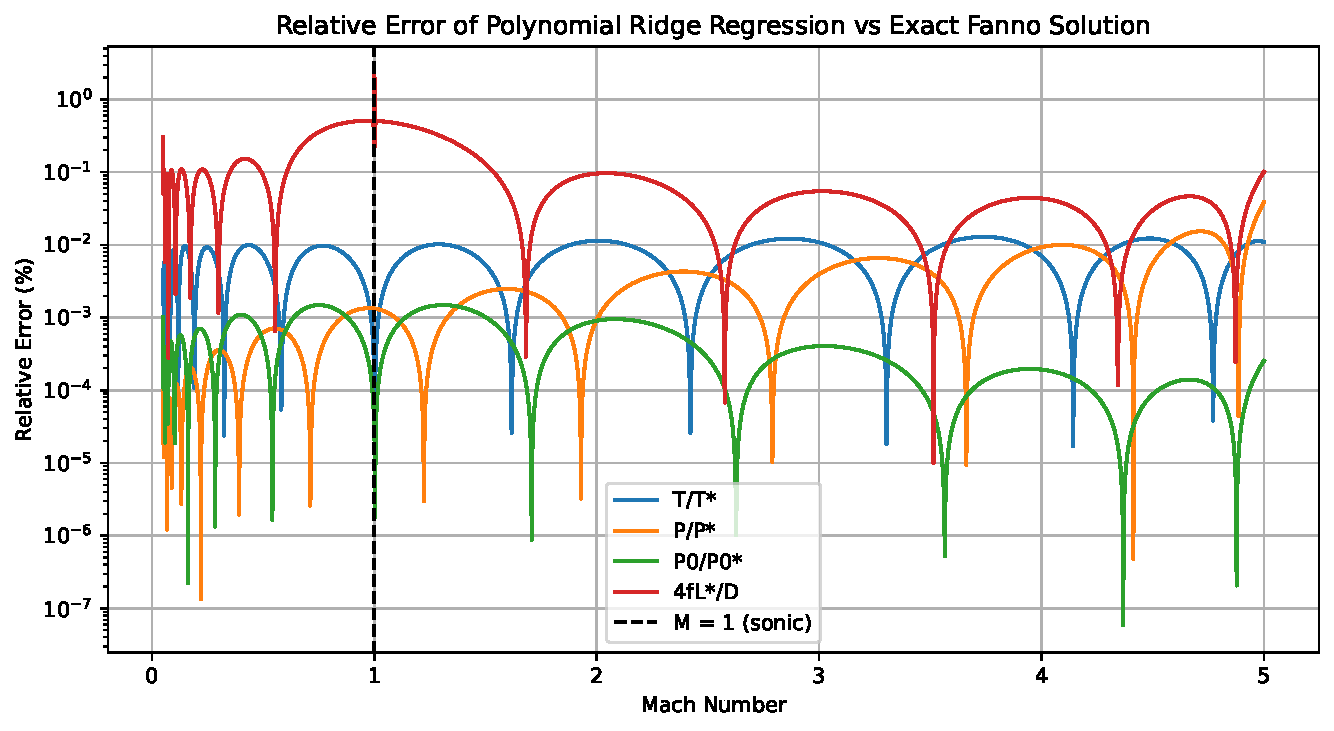
\includegraphics[width=0.85\textwidth]{fig_poly_ridge_error.pdf}
\caption{Relative error of the third-degree Polynomial Ridge Regression predictions compared to the exact Fanno solution. The relative error is computed using $\varepsilon_\mathrm{rel} = 100 \, |\hat{y}-y|/y$. The vertical dashed line indicates the sonic point ($M=1$), where the Fanno function exhibits singular behavior. The plot shows that the model predicts all outputs accurately across most of the Mach range, with slightly larger errors near $M=1$.}
\label{fig:poly_ridge_error}
\end{figure}


\paragraph{Representative Mach Numbers --- Table Comparison}
Tables~\ref{tab:ml_vs_exact_1} and \ref{tab:ml_vs_exact_2} summarize the predictive performance of the third-degree Polynomial Ridge Regression model at selected Mach numbers spanning subsonic, sonic, and supersonic regimes. Table~\ref{tab:ml_vs_exact_1} presents the temperature and pressure ratios ($T/T^*$, $P/P^*$), while Table~\ref{tab:ml_vs_exact_2} reports the total pressure ratio ($P_0/P_0^*$) and the normalized friction length ($4fL^*/D$). The ML predictions closely match the exact Fanno flow values across nearly all Mach numbers, demonstrating the high fidelity of the regression model. Small deviations are observed near the sonic point ($M = 1$), consistent with the singular behavior of the Fanno flow relations, particularly in variables that approach zero or have steep derivatives. Overall, these results provide a quantitative benchmark for the model before evaluating more advanced neural network and physics-informed approaches.

\begin{table}[htbp]
\centering
\small
\setlength{\tabcolsep}{6pt}
\renewcommand{\arraystretch}{1.1}
\caption{Polynomial Ridge regression versus exact Fanno solution for $T/T^*$ and $P/P^*$ at selected Mach numbers.}
\label{tab:ml_vs_exact_1}
\begin{tabular}{@{} c rr rr @{}}
\toprule
 & \multicolumn{2}{c}{$T/T^*$} & \multicolumn{2}{c}{$P/P^*$} \\
\cmidrule(lr){2-3} \cmidrule(lr){4-5}
$M$ & {Exact} & {Poly-Ridge} & {Exact} & {Poly-Ridge} \\
\midrule
0.3 & 1.178782 & 1.178830 & 3.619057 & 3.619044 \\
0.6 & 1.119403 & 1.119422 & 1.763364 & 1.763375 \\
1.0 & 1.000000 & 1.000001 & 1.000000 & 0.999987 \\
1.5 & 0.827586 & 0.827542 & 0.606478 & 0.606492 \\
2.5 & 0.533333 & 0.533315 & 0.292119 & 0.292107 \\
3.0 & 0.428571 & 0.428525 & 0.218218 & 0.218227 \\
\bottomrule
\end{tabular}
\end{table}

\begin{table}[htbp]
\centering
\small
\setlength{\tabcolsep}{6pt}
\renewcommand{\arraystretch}{1.1}
\caption{Polynomial Ridge regression versus exact Fanno solution for $P_0/P_0^*$ and $4fL^*/D$ at selected Mach numbers.}
\label{tab:ml_vs_exact_2}
\begin{tabular}{@{} c rr rr @{}}
\toprule
 & \multicolumn{2}{c}{$P_0/P_0^*$} & \multicolumn{2}{c}{$4fL^*/D$} \\
\cmidrule(lr){2-3} \cmidrule(lr){4-5}
$M$ & {Exact} & {Poly-Ridge} & {Exact} & {Poly-Ridge} \\
\midrule
0.3 & 2.035065 & 2.035060 & 5.299253 & 5.299454 \\
0.6 & 1.188200 & 1.188207 & 0.490822 & 0.490389 \\
1.0 & 1.000000 & 1.000000 & 0.000000 & 0.000000 \\
1.5 & 1.176167 & 1.176155 & 0.136050 & 0.135873 \\
2.5 & 2.636719 & 2.636726 & 0.431977 & 0.432053 \\
3.0 & 4.234568 & 4.234551 & 0.522159 & 0.521874 \\
\bottomrule
\end{tabular}
\end{table}


Figure~\ref{fig:poly_ridge_nn_vs_exact} compares the Polynomial Ridge regression predictions with the exact Fanno flow values across all Mach numbers. All ML predictions are shown as thick red lines, while the exact solutions are black dashed lines. The model demonstrates excellent agreement over the entire range, capturing the subsonic and supersonic trends accurately. Minor deviations occur in $4fL^*/D$ near the sonic point ($M=1$), reflecting the singular behavior of the governing equations rather than a deficiency of the regression model.

\begin{figure}[h!]
\centering
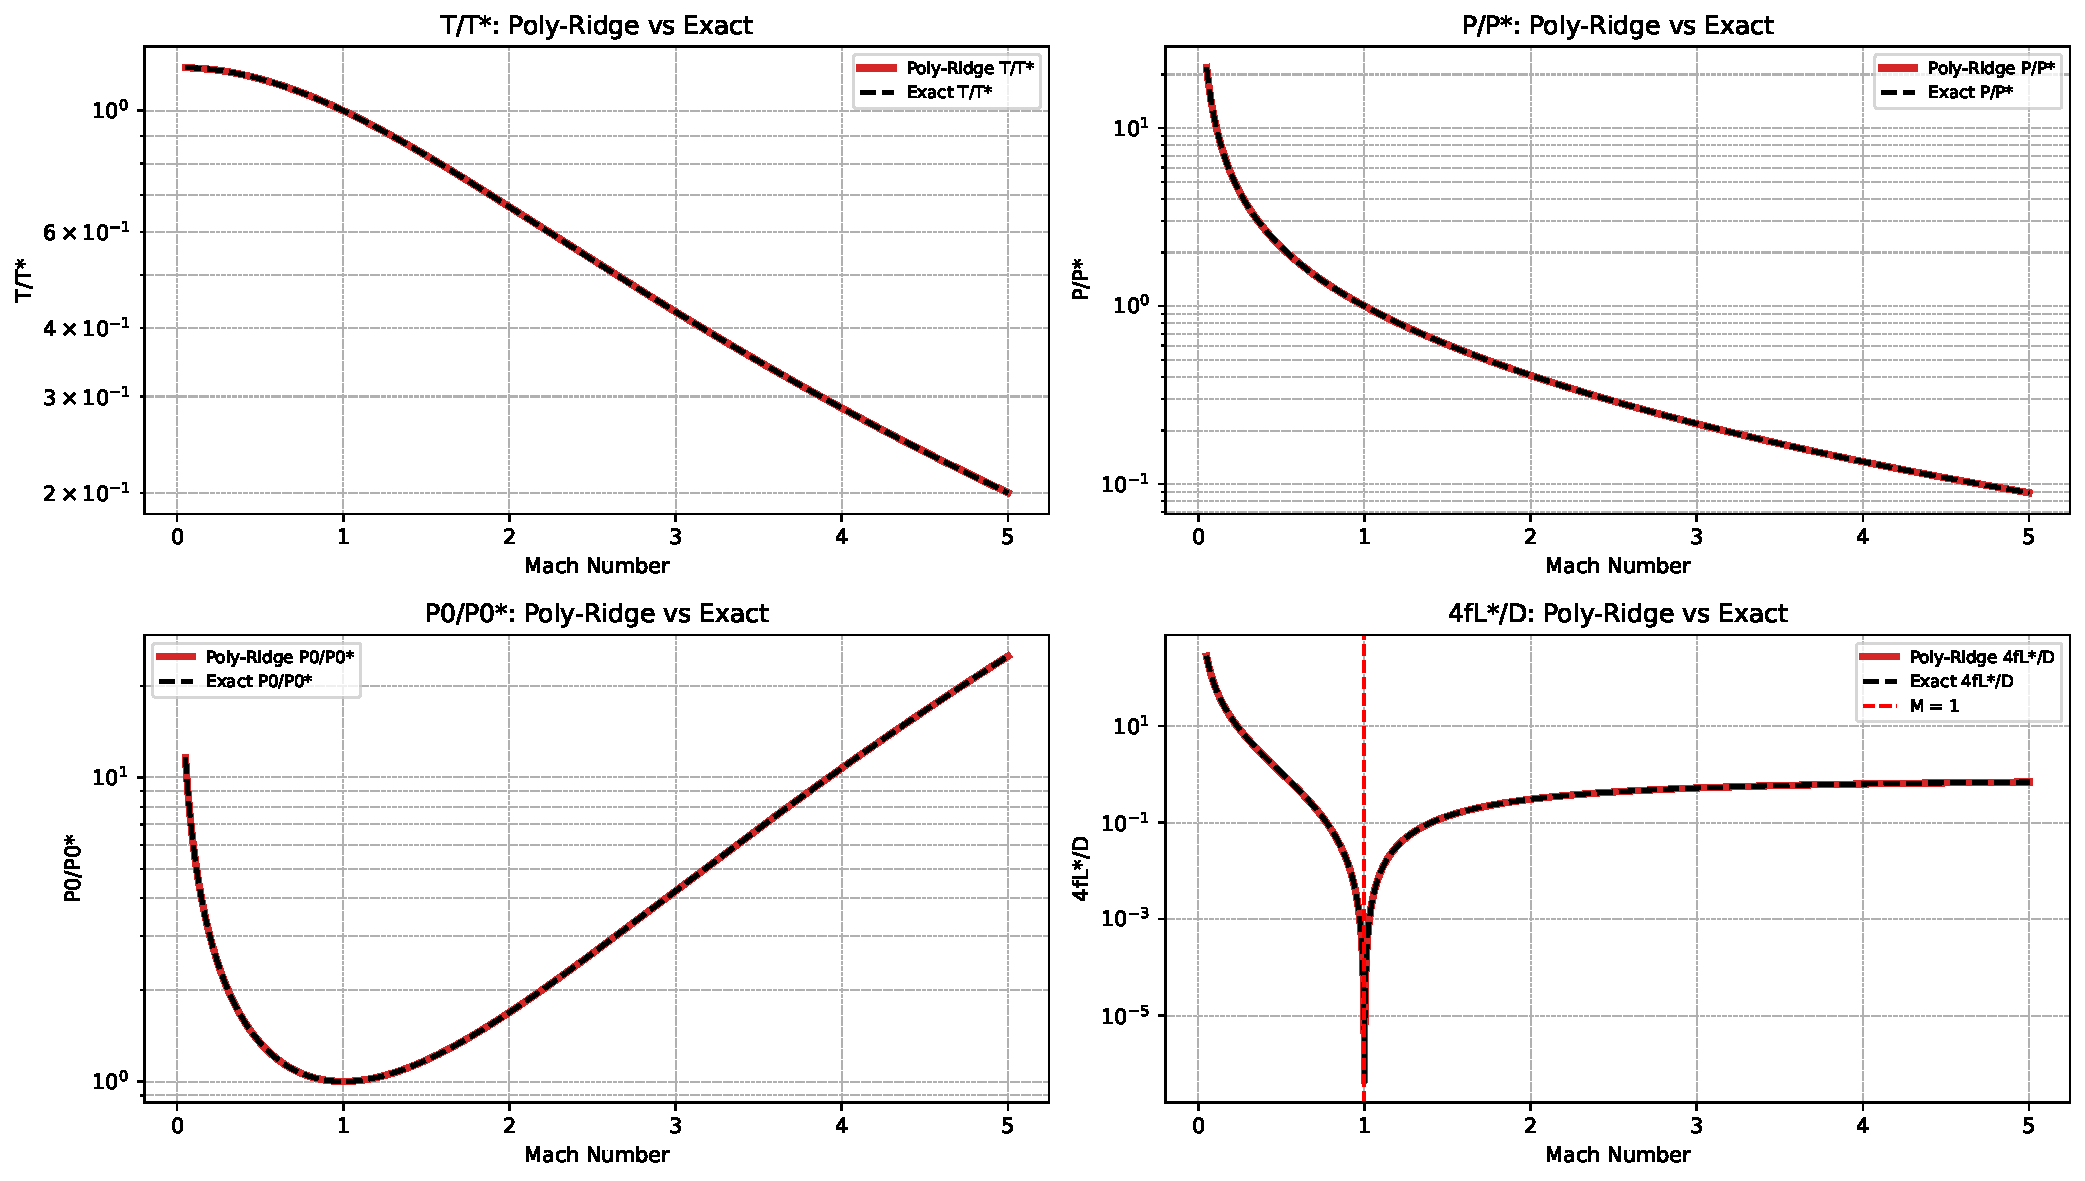
\includegraphics[width=0.95\textwidth]{fig_poly_ridge_all_outputs.pdf}
\caption{Comparison of Polynomial Ridge regression predictions (thick red lines) with exact Fanno flow values (black dashed lines) for $T/T^*$, $P/P^*$, $P_0/P_0^*$, and $4fL^*/D$. Deviations near the sonic point ($M=1$) are visible, particularly for $4fL^*/D$.}
\label{fig:poly_ridge_nn_vs_exact}
\end{figure}



The results demonstrate how classical regression can be used to accurately approximate the Fanno flow relations. A key factor in the high performance observed here is the feature engineering: since the exact solution was known, we were able to construct features ($M^2$, $1/M$, $1/M^2$, $\log M$) that directly capture the nonlinear, reciprocal, and logarithmic behaviors of the governing equations. In practical applications where the exact solution is unknown, feature selection or engineering may not be as straightforward, and the predictive performance of classical regression models could be substantially lower. Nevertheless, this example provides a practical template for applying data-driven surrogate modeling to more complex or computationally intensive gas dynamics problems, where well-chosen features can significantly enhance model accuracy and generalization across multiple outputs.


\subsection{Forward Surrogate Neural Network for Fanno Flow}

The Polynomial Ridge regression model captures the Fanno relations to high accuracy, but its success relied on a deliberate choice of physics-engineered features. In more demanding settings---high-dimensional parametric studies, variable duct geometries, or coupled flow--thermal phenomena---closed-form features may not be available, and the regression fit becomes correspondingly less reliable. A natural next step is to replace the polynomial regressor with a feedforward neural network and let the network discover its own internal representation of the nonlinearities.

In the language used throughout this chapter, the network is a \emph{forward surrogate}: \emph{forward} because it takes inlet or boundary conditions as input and returns flow properties as output (the same direction as the analytical Fanno solver), and \emph{surrogate} because, once trained, it stands in for that solver and evaluates each query at the cost of a single forward pass. Neural-network surrogates of this form are now standard in fluid dynamics for parametric and real-time applications \cite{Duraisamy2019, Brunton2020}.

\subsubsection{Key Components of a Forward Surrogate Model}

A typical forward surrogate neural network has the following elements:

\begin{enumerate}
    \item \textbf{Inputs:} Quantities that define the flow. For the Fanno flow problem, inputs include:
    \begin{itemize}
        \item Mach number, $M$,
        \item Derived features such as $M^2$, $1/M$, $1/M^2$, and $\ln(M)$, which help the network capture nonlinear relationships.
    \end{itemize}
    
    \item \textbf{Hidden Layers:} Intermediate computational layers that combine weighted inputs with nonlinear activation functions. Multiple hidden layers allow the network to approximate highly nonlinear functions, such as the Fanno relation.
    
    \item \textbf{Outputs:} Flow properties predicted by the network:
    \begin{itemize}
        \item Normalized temperature $T/T^*$,
        \item Static pressure $P/P^*$,
        \item Stagnation pressure $P_0/P_0^*$,
        \item Cumulative friction parameter $4 f L^*/D$.
    \end{itemize}
    
    \item \textbf{Training Process:} The network learns by comparing its predictions to exact values from the Fanno equations. The difference is quantified using a \emph{loss function}, such as mean squared error (MSE). The network adjusts its internal weights to reduce this error over many iterations.
\end{enumerate}

\subsubsection{How to Build a Forward Surrogate for Fanno Flow}

The process of constructing a forward surrogate neural network can be summarized in six steps. These steps correspond directly to the components illustrated in Figure~\ref{fig:surrogate_nn}, where the input features, hidden layers, and output nodes are shown schematically.

\begin{figure}[h!]
\centering
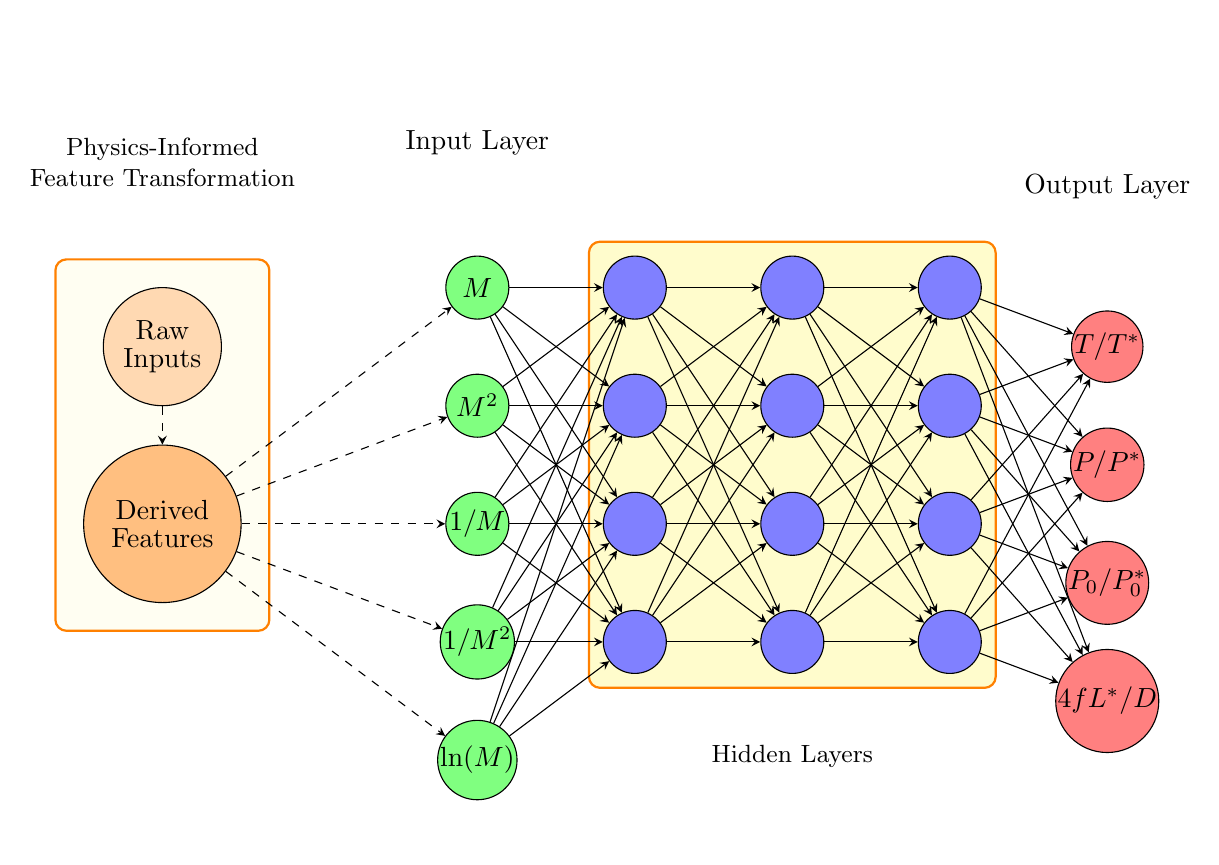
\begin{tikzpicture}[x=2.0cm, y=1.5cm, >=stealth,
every node/.style={circle, draw, minimum size=8mm, inner sep=0pt}]

% ====== Feature Engineering Layer ======
\node[fill=orange!30, minimum size=15mm] (F_raw) at (-2,0) {\shortstack{Raw \\Inputs }};
\node[fill=orange!50, minimum size=20mm] (F_derived) at (-2,-1.5) {\shortstack{Derived \\Features }};

% ====== Box for Physics-Informed Transformation ======
\begin{pgfonlayer}{background}
\node[fill=yellow!5, draw=orange, thick,
      fit=(F_raw)(F_derived), 
      inner sep=10pt, 
      rounded corners, 
      rectangle,
      label={[font=\small, align=center, yshift=-5mm]above:Physics-Informed\\Feature Transformation}] (featbox) {};
\end{pgfonlayer}

% ====== Input Layer ======
\node[fill=green!50] (I1) at (0,0.5) {$M$};
\node[fill=green!50] (I2) at (0,-0.5) {$M^2$};
\node[fill=green!50] (I3) at (0,-1.5) {$1/M$};
\node[fill=green!50] (I4) at (0,-2.5) {$1/M^2$};
\node[fill=green!50] (I5) at (0,-3.5) {$\ln(M)$};
\node[draw=none, fill=none, above=0.5cm of I1] {Input Layer};

% ====== Hidden Layer 1 ======
\node[fill=blue!50] (H1_1) at (1,0.5) {};
\node[fill=blue!50] (H1_2) at (1,-0.5) {};
\node[fill=blue!50] (H1_3) at (1,-1.5) {};
\node[fill=blue!50] (H1_4) at (1,-2.5) {};

% ====== Hidden Layer 2 ======
\node[fill=blue!50] (H2_1) at (2,0.5) {};
\node[fill=blue!50] (H2_2) at (2,-0.5) {};
\node[fill=blue!50] (H2_3) at (2,-1.5) {};
\node[fill=blue!50] (H2_4) at (2,-2.5) {};

% ====== Hidden Layer 3 ======
\node[fill=blue!50] (H3_1) at (3,0.5) {};
\node[fill=blue!50] (H3_2) at (3,-0.5) {};
\node[fill=blue!50] (H3_3) at (3,-1.5) {};
\node[fill=blue!50] (H3_4) at (3,-2.5) {};

% ====== Background rectangle for Hidden Layers ======
\begin{pgfonlayer}{background}
\node[fill=yellow!20, draw=orange, thick,
fit=(H1_1)(H1_4)(H2_1)(H2_4)(H3_1)(H3_4), inner sep=5pt, rounded corners, rectangle] {};
\end{pgfonlayer}

% ====== Hidden Layer Label ======
\node[draw=none, fill=none, font=\small, below=4.5cm of H2_1] {Hidden Layers};

% ====== Output Layer ======
\node[fill=red!50] (O1) at (4,0) {$T/T^*$};
\node[fill=red!50] (O2) at (4,-1) {$P/P^*$};
\node[fill=red!50] (O3) at (4,-2) {$P_0/P_0^*$};
\node[fill=red!50] (O4) at (4,-3) {$4 f L^*/D$};
\node[draw=none, fill=none, above=0.5cm of O1] {Output Layer};

% ====== Connections ======
% Derived Features -> Input Layer
\foreach \j in {1,...,5}
    \draw[->, dashed] (F_derived) -- (I\j);

% Input -> Hidden 1
\foreach \i in {1,...,5}
    \foreach \j in {1,...,4}
        \draw[->] (I\i) -- (H1_\j);

% Hidden 1 -> Hidden 2
\foreach \i in {1,...,4}
    \foreach \j in {1,...,4}
        \draw[->] (H1_\i) -- (H2_\j);

% Hidden 2 -> Hidden 3
\foreach \i in {1,...,4}
    \foreach \j in {1,...,4}
        \draw[->] (H2_\i) -- (H3_\j);

% Hidden 3 -> Output
\foreach \i in {1,...,4}
    \foreach \j in {1,...,4}
        \draw[->] (H3_\i) -- (O\j);

% Raw Inputs -> Derived Features
\draw[->, dashed] (F_raw) -- (F_derived);

\end{tikzpicture}
\caption{Forward surrogate neural network for Fanno flow prediction. Raw input $M$ and derived features ($M^2$, $1/M$, $1/M^2$, $\ln M$) are enclosed in the orange box labelled ``Physics-Informed Feature Transformation'' to indicate that feature engineering is guided by the analytical structure of the Fanno relation. The engineered features feed the network input layer (green). Three hidden layers (blue) capture nonlinear dependencies, and the output layer (red) returns the four normalized flow quantities $T/T^*$, $P/P^*$, $P_0/P_0^*$, and $4 f L^*/D$. Dashed arrows denote feature-engineering preprocessing; solid arrows denote learned network connections.}
\label{fig:surrogate_nn}
\end{figure}

\paragraph{Data, Features, and Scaling (Steps 1--3)}
The dataset is generated by sampling Mach numbers across the subsonic and supersonic regimes and evaluating the Fanno function for each, producing analytical labels for $T/T^{\ast}$, $P/P^{\ast}$, $P_{0}/P_{0}^{\ast}$, and $4 f L^{\ast}/D$. Each input vector is augmented with the same engineered features used by the regression baseline, $\mathbf{x} = [M,\, M^{2},\, 1/M,\, 1/M^{2},\, \ln M]^{T}$, and both inputs and outputs are then standardized to zero mean and unit variance so that the optimizer treats heterogeneous scales uniformly.

\paragraph{Architecture, Training, and Validation (Steps 4--6)}
The network of Figure~\ref{fig:surrogate_nn} uses three hidden layers with nonlinear activations, an input layer matching the engineered feature vector, and four output nodes for the flow ratios. Training minimizes the mean squared error between predicted and analytical labels using the Adam optimizer \cite{Kingma2015Adam} together with early stopping on a held-out validation set \cite{Prechelt1998} to prevent overfitting. Predictive accuracy is reported as the relative error
\[
\varepsilon_{\mathrm{rel}}\,(\%) \;=\; 100 \times \frac{|\,\hat{y} - y\,|}{|\,y\,|},
\]
where $y$ is the analytical Fanno value and $\hat{y}$ the network prediction.

\paragraph{Results}
Figures~\ref{fig:nn_all_outputs} and~\ref{fig:nn_error} summarize the surrogate network's predictive performance. The network reproduces all four flow quantities with high fidelity over the full Mach number range, and the relative error remains below $1.2\%$ everywhere, with the worst point lying near the sonic limit where $4fL^{*}/D$ vanishes and the relative-error metric becomes ill-defined. Table~\ref{tab:nn_vs_exact} reports a quantitative comparison at representative subsonic, sonic, and supersonic Mach numbers for the total-pressure ratio and the friction parameter; agreement is consistent to four or more significant digits across all outputs.

\begin{figure}[h!]
\centering
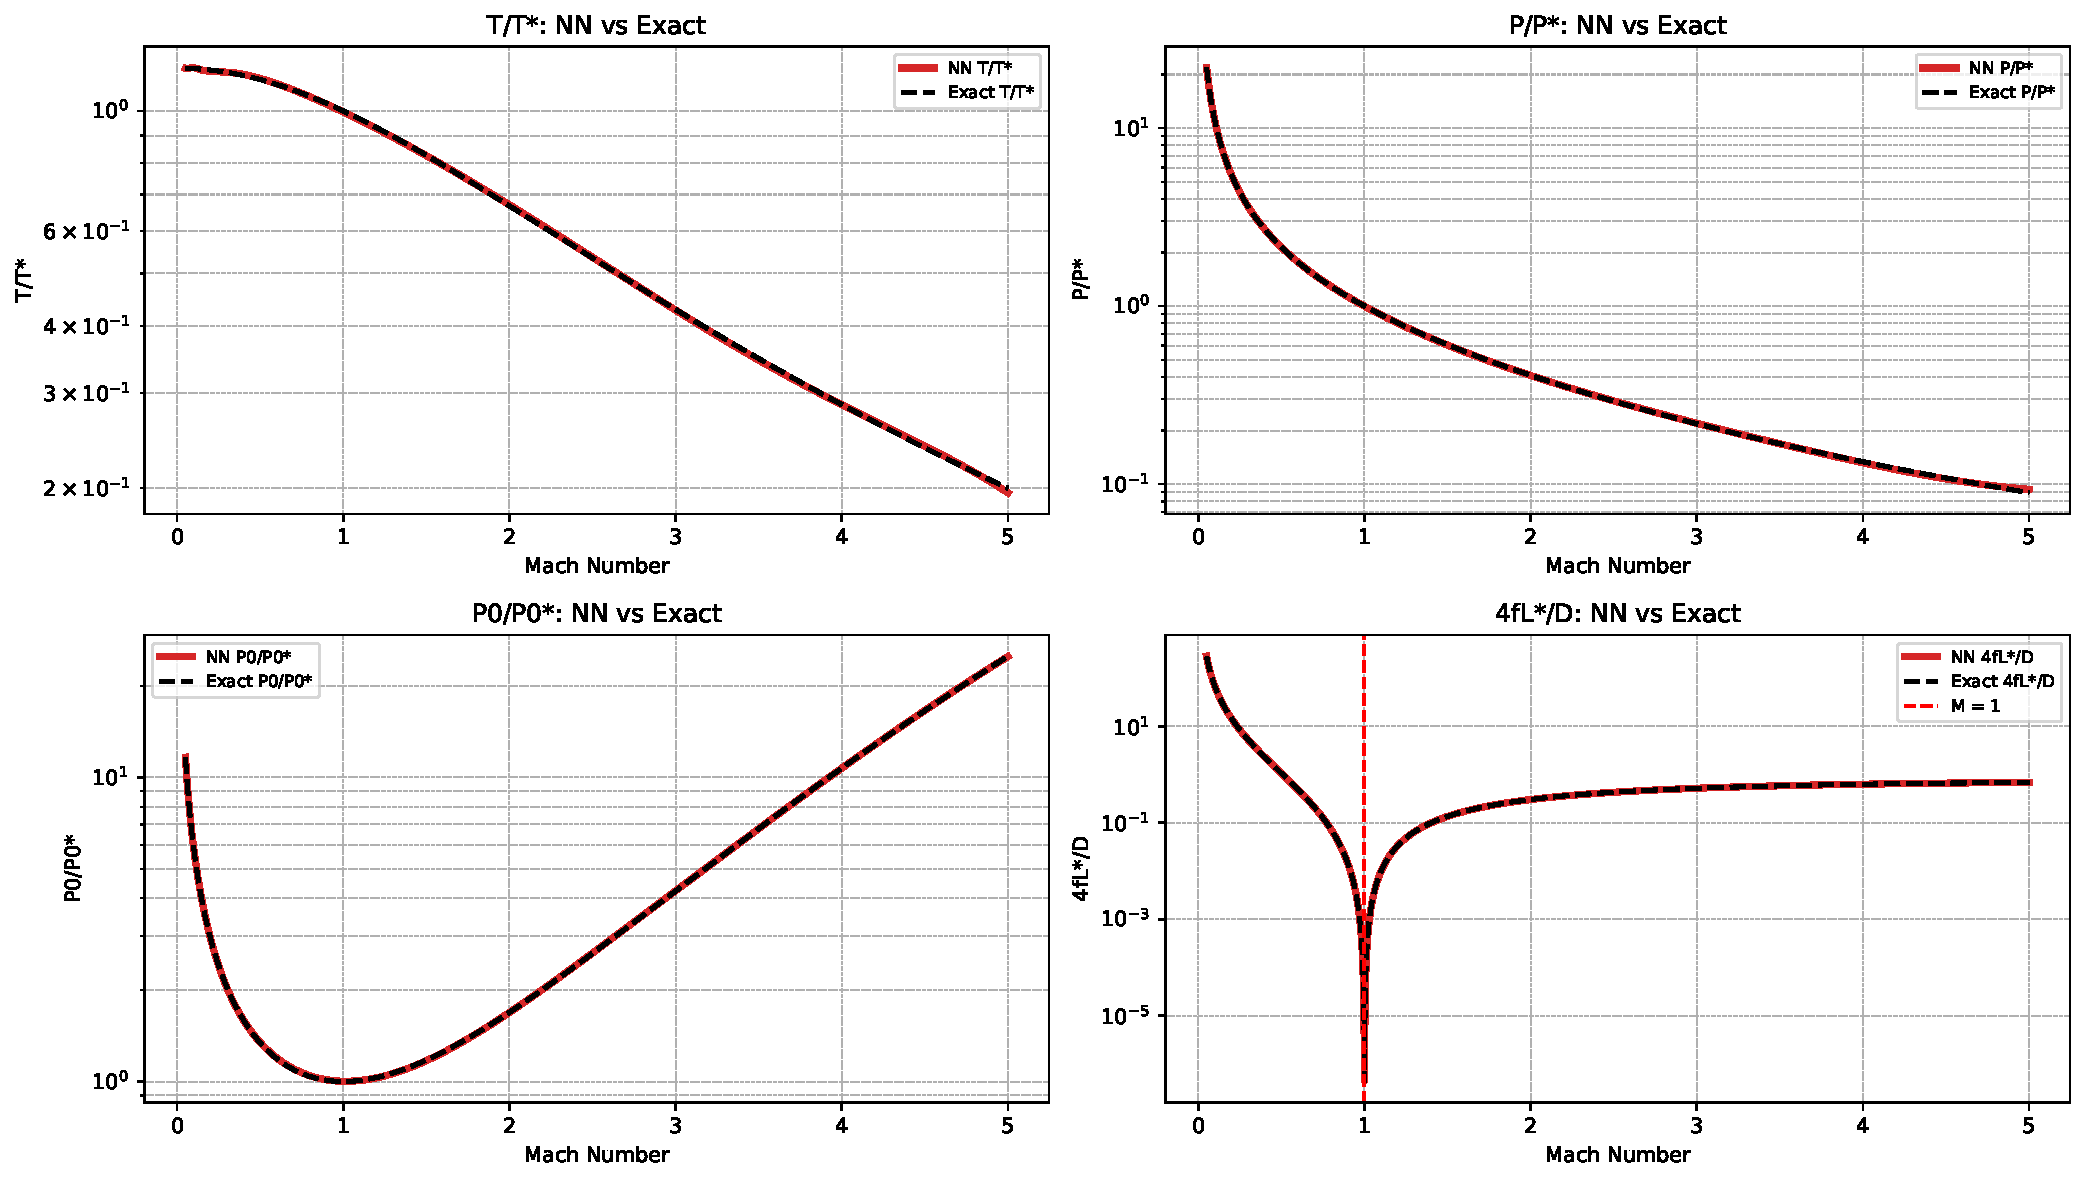
\includegraphics[width=0.95\textwidth]{fig_nn_all_outputs.pdf}
\caption{Surrogate neural network predictions (thick red lines) versus exact Fanno flow values (black dashed lines) for $T/T^*$, $P/P^*$, $P_0/P_0^*$, and $4fL^*/D$. The network is trained on physics-informed engineered features $[M, M^2, 1/M, 1/M^2, \ln M]$ and predicts all four normalized flow quantities simultaneously. The vertical dashed line in the friction-length panel marks the sonic point.}
\label{fig:nn_all_outputs}
\end{figure}

\begin{figure}[h!]
\centering
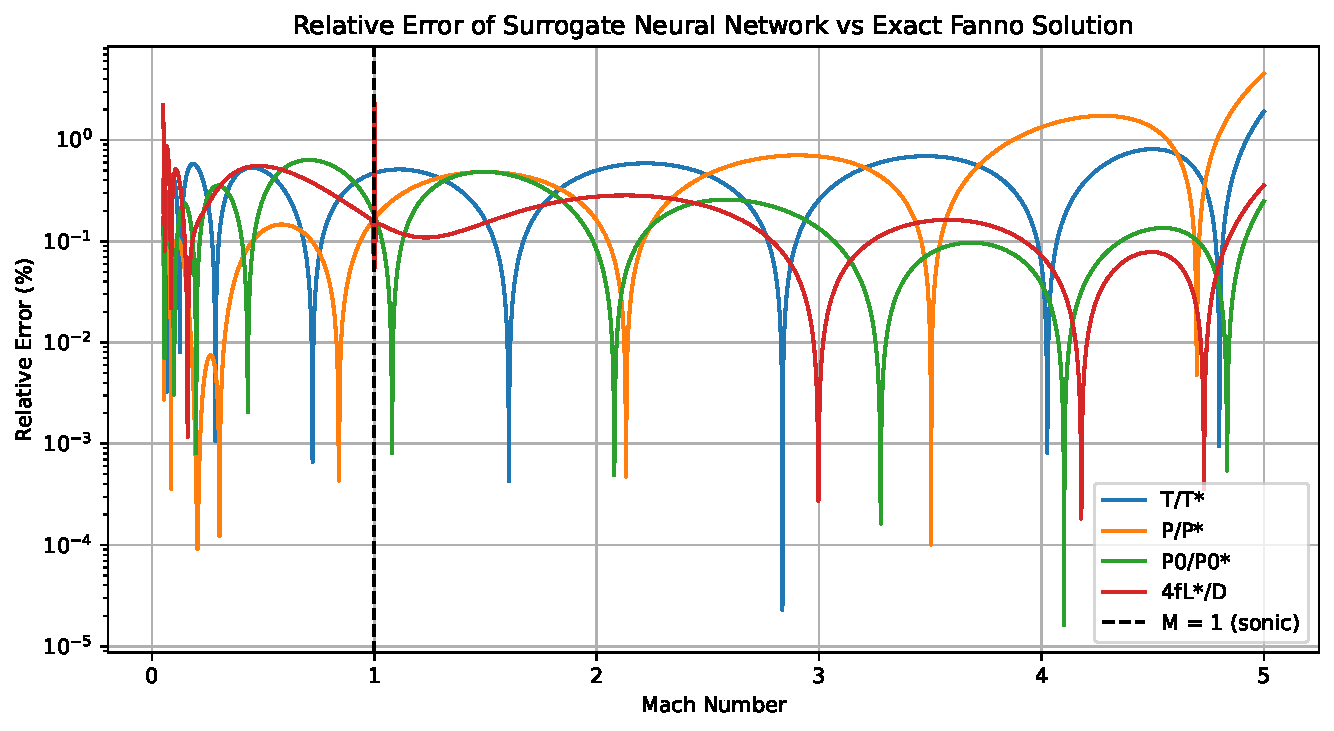
\includegraphics[width=0.85\textwidth]{fig_nn_error.pdf}
\caption{Relative error (logarithmic scale) of the surrogate neural network compared to the exact Fanno solution. The vertical dashed line indicates the sonic point ($M=1$), where $4fL^*/D$ vanishes and the relative error metric becomes ill-defined.}
\label{fig:nn_error}
\end{figure}

\begin{figure}[h!]
\centering
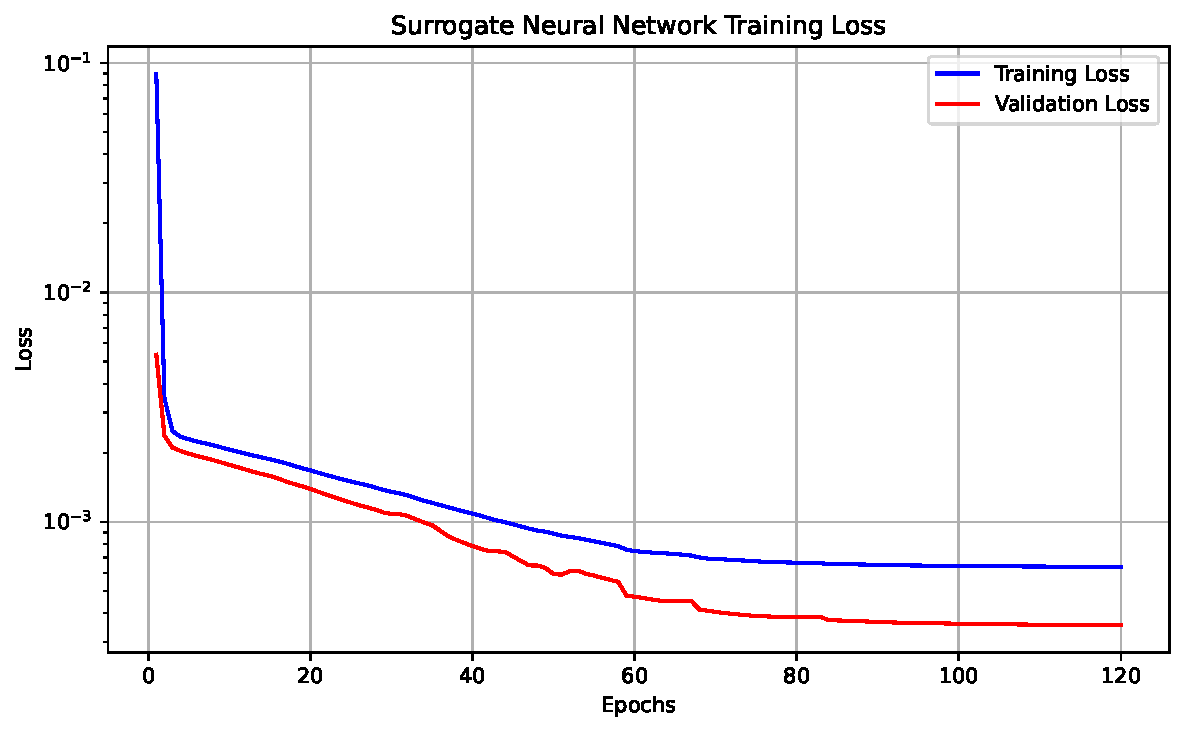
\includegraphics[width=0.7\textwidth]{fig_nn_loss_history.pdf}
\caption{Surrogate neural network training and validation loss versus epoch (logarithmic scale). The smooth, monotonic decrease followed by a plateau is the expected signature of a well-conditioned supervised regression problem on a noise-free analytical dataset.}
\label{fig:nn_loss_history}
\end{figure}

\begin{table}[h!]
\centering
\small
\caption{Surrogate neural network predictions versus exact Fanno values for $P_{0}/P_{0}^{\ast}$ and $4 f L^{\ast}/D$ at representative Mach numbers.}
\label{tab:nn_vs_exact}
\begin{tabular}{c|cc|cc}
\hline
$M$ & $P_0/P_0^*$ exact & $P_0/P_0^*$ NN & $4fL^*/D$ exact & $4fL^*/D$ NN \\
\hline
0.3 & 2.03507 & 2.02783 & 5.29925 & 5.28143 \\
0.6 & 1.18820 & 1.19459 & 0.49082 & 0.48839 \\
1.0 & 1.00000 & 1.00181 & 0.00000 & 0.00000 \\
1.5 & 1.17617 & 1.17046 & 0.13605 & 0.13584 \\
2.5 & 2.63672 & 2.64334 & 0.43198 & 0.43103 \\
3.0 & 4.23457 & 4.24021 & 0.52216 & 0.52217 \\
\hline
\end{tabular}
\end{table}

\subsection{Physics-Informed Neural Networks for Fanno Flow}
Having addressed Fanno flow with classical regression and with a supervised surrogate neural network, we now turn to a \textbf{Physics-Informed Neural Network (PINN)}. The previous two methods are data-driven: the model is fit to a list of $(M, F)$ pairs and the governing equations are used only indirectly, to generate that list. A PINN reverses this relationship by placing the governing equations \emph{inside} the training objective, so that the neural network's output is constrained to satisfy the Fanno ODE at every point queried during training. The result is a continuous, differentiable approximation that respects the physics by construction rather than by interpolation.

\subsubsection{Motivation for PINNs}
The transition from classical regression and surrogate neural networks to physics-informed neural networks (PINNs) is motivated by limitations of the previous approaches:

\begin{itemize}
    \item \textbf{Classical regression.} Polynomial Ridge regression with physics-engineered features captures the Fanno function accurately on the sampled Mach number range, but the model is purely empirical: nothing in its construction prevents it from violating the governing ODE outside the training distribution. It also requires the analytical structure of the solution to be known a priori in order to design the input features.
    \item \textbf{Forward surrogate neural network.} The supervised neural network removes the need for hand-engineered features and produces smooth multi-output predictions, but it is still trained on labelled data and inherits the same fundamental weakness: there is no structural reason for the predictions to satisfy the underlying conservation laws when the network is queried far from its training points.
\end{itemize}

Physics-informed neural networks address these limitations by placing the governing \textbf{ODE} directly inside the training objective. The cumulative friction parameter $4 f L^{*}/D$ is then constrained to satisfy the Fanno equation at every collocation point evaluated during training, regardless of whether labelled data are available there.

\subsubsection{PINN Concept}
A PINN is a neural network whose output is trained to satisfy a differential equation rather than a list of input--output pairs. Its defining feature is that the \textbf{ODE residual} (computed from the network's own output via automatic differentiation) appears directly in the loss function. The training signal is therefore the physical law itself, and labelled data are optional rather than essential.

For the Fanno problem, a single-input single-output network $\hat{F}_{\theta}(M)$ approximates $F(M) = 4fL^*/D$. At every iteration the network is queried at a batch of collocation points $\{M_i\}_{i=1}^{N_c}$; automatic differentiation produces $d\hat{F}/dM$ at the same points; the difference between the network derivative and the analytical right-hand side of the ODE is squared and minimized. The boundary condition is imposed either as an additional penalty term or, as we do here, exactly through an output transformation. In this way the physics is embedded directly into the gradient flow of the optimizer rather than being inferred indirectly from labelled examples.

\subsubsection{Construction of a PINN for Fanno Flow}
The Fanno function $\Phi(M)$ defined in the previous sections is itself an antiderivative: the right-hand side of the ODE follows from differentiating the closed-form expression for $\Phi$ with respect to $M$ and simplifying. The result is a compact rational expression,

\begin{equation}
\label{eq:fanno_ode}
\frac{dF}{dM} \;=\; \mathrm{RHS}(M) \;\equiv\; \frac{4\,(M^{2}-1)}{\gamma\,M^{3}\left[\,2+(\gamma-1)M^{2}\,\right]}, \qquad F(1) = 0.
\end{equation}

The boundary condition $F(1) = 0$ is the \emph{sonic anchor} of Fanno flow: the duct length required to reach the sonic state vanishes when the flow is already sonic. Note that $\mathrm{RHS}(M)$ is negative for $M < 1$, zero at $M = 1$, and positive for $M > 1$; the function $F(M)$ therefore has a minimum at the sonic point. Once $F(M)$ has been learned, the auxiliary flow variables $T/T^*$, $P/P^*$, and $P_0/P_0^*$ are recovered from the analytical Fanno relations, since each is a closed-form function of $M$ alone for a calorically perfect gas.

\paragraph{Network Architecture}
The PINN used in this chapter is a small, fully connected network with the following structure:

\begin{itemize}
    \item \textbf{Input.} Mach number $M$ (one scalar). It is normalized to $[-1, 1]$ before entering the first hidden layer to keep the activation regime well conditioned.
    \item \textbf{Hidden layers.} Four fully connected layers of $64$ neurons each, with $\tanh$ activations \cite{Goodfellow2016}. The choice of $\tanh$ is motivated by the need for smooth, differentiable nonlinearities so that automatic differentiation produces accurate first derivatives; alternative smooth activations such as Swish \cite{Ramachandran2017} or learnable adaptive activations \cite{Jagtap2020} are equally suitable.
    \item \textbf{Output transformation.} A single linear neuron returns an internal scalar $g_{\theta}(M)$. The final prediction is $\hat{F}(M) = (M-1)\,g_{\theta}(M)$, which guarantees $\hat{F}(1) = 0$ by construction. This is the \emph{hard boundary condition} trick and removes the need for a separate BC penalty term.
\end{itemize}

\paragraph{Loss Function}
With the hard BC built into the architecture, the only remaining requirement is that $\hat{F}$ satisfy the ODE. The loss is therefore a pure ODE-residual loss,

\begin{equation}
\label{eq:pinn_loss}
\mathcal{L}_{\mathrm{PINN}} \;=\; \frac{1}{N_c} \sum_{i=1}^{N_c}
\left[
\frac{1}{|\mathrm{RHS}(M_i)| + 1}\left(\frac{d\hat{F}}{dM}\bigg|_{M_i} - \mathrm{RHS}(M_i)\right)
\right]^{2},
\end{equation}

where the prefactor $1/(|\mathrm{RHS}(M_i)| + 1)$ rescales the residual at each collocation point. This rescaling is necessary because $\mathrm{RHS}(M)$ varies over more than three orders of magnitude across the Mach domain (from $\sim\!10^{3}$ in magnitude at $M = 0.1$ to $\sim\!10^{-2}$ at $M = 5$); without it, the unscaled mean-squared error would be entirely dominated by the small-$M$ stiff region and the optimizer would never converge on the supersonic branch. After scaling, every collocation point contributes a residual of order unity, so the gradient updates balance the two regimes naturally. \textbf{No labelled $(M, F)$ data are used in this loss}; the network learns $F(M)$ entirely from the ODE itself.

\paragraph{Training Procedure}
Training proceeds with the Adam optimizer \cite{Kingma2015Adam} and a piecewise-constant learning-rate schedule (initial rate $2\times 10^{-3}$, decayed in three stages to $3\times 10^{-5}$ over $8000$ epochs). Each training step consists of:
\begin{enumerate}
    \item Resample $N_c$ collocation points: half log-uniform in $M \in [0.1, 0.97]$ (placing more density in the stiff $M\!\to\!0$ region) and half uniform in $M \in [1.03, 5.0]$. The narrow band around $M = 1$ is excluded to avoid the $1/M^3$ singularity in the analytical RHS.
    \item Forward pass: evaluate $\hat{F}(M_i)$ at every collocation point.
    \item Inner gradient tape: compute $d\hat{F}/dM\big|_{M_i}$ by automatic differentiation.
    \item Outer gradient tape: evaluate $\mathcal{L}_{\mathrm{PINN}}$ and backpropagate to update the network weights.
\end{enumerate}
Because the physics is embedded in the loss, the network generalizes smoothly across the entire Mach range, including in regions where dense labelled data are unavailable.

\paragraph{Post-Processing and Validation}
Once the PINN has been trained, the solution must be validated systematically. The post-processing workflow involves three complementary checks: visual comparison against the exact solution, quantitative inspection of the relative error, and analysis of the training history.

\paragraph{Comparison with the Exact Solution}
Figure~\ref{fig:pinn_all_outputs} compares the PINN-predicted flow quantities with the analytical Fanno solution over the full Mach number range. The temperature, pressure, and total-pressure ratios are reconstructed analytically from $M$ and therefore match the exact curves to machine precision. The cumulative friction parameter $4fL^*/D$ is the actual learned output of the PINN, and its agreement with the exact Fanno function confirms that the ODE has been integrated correctly by the network.

\begin{figure}[h!]
\centering
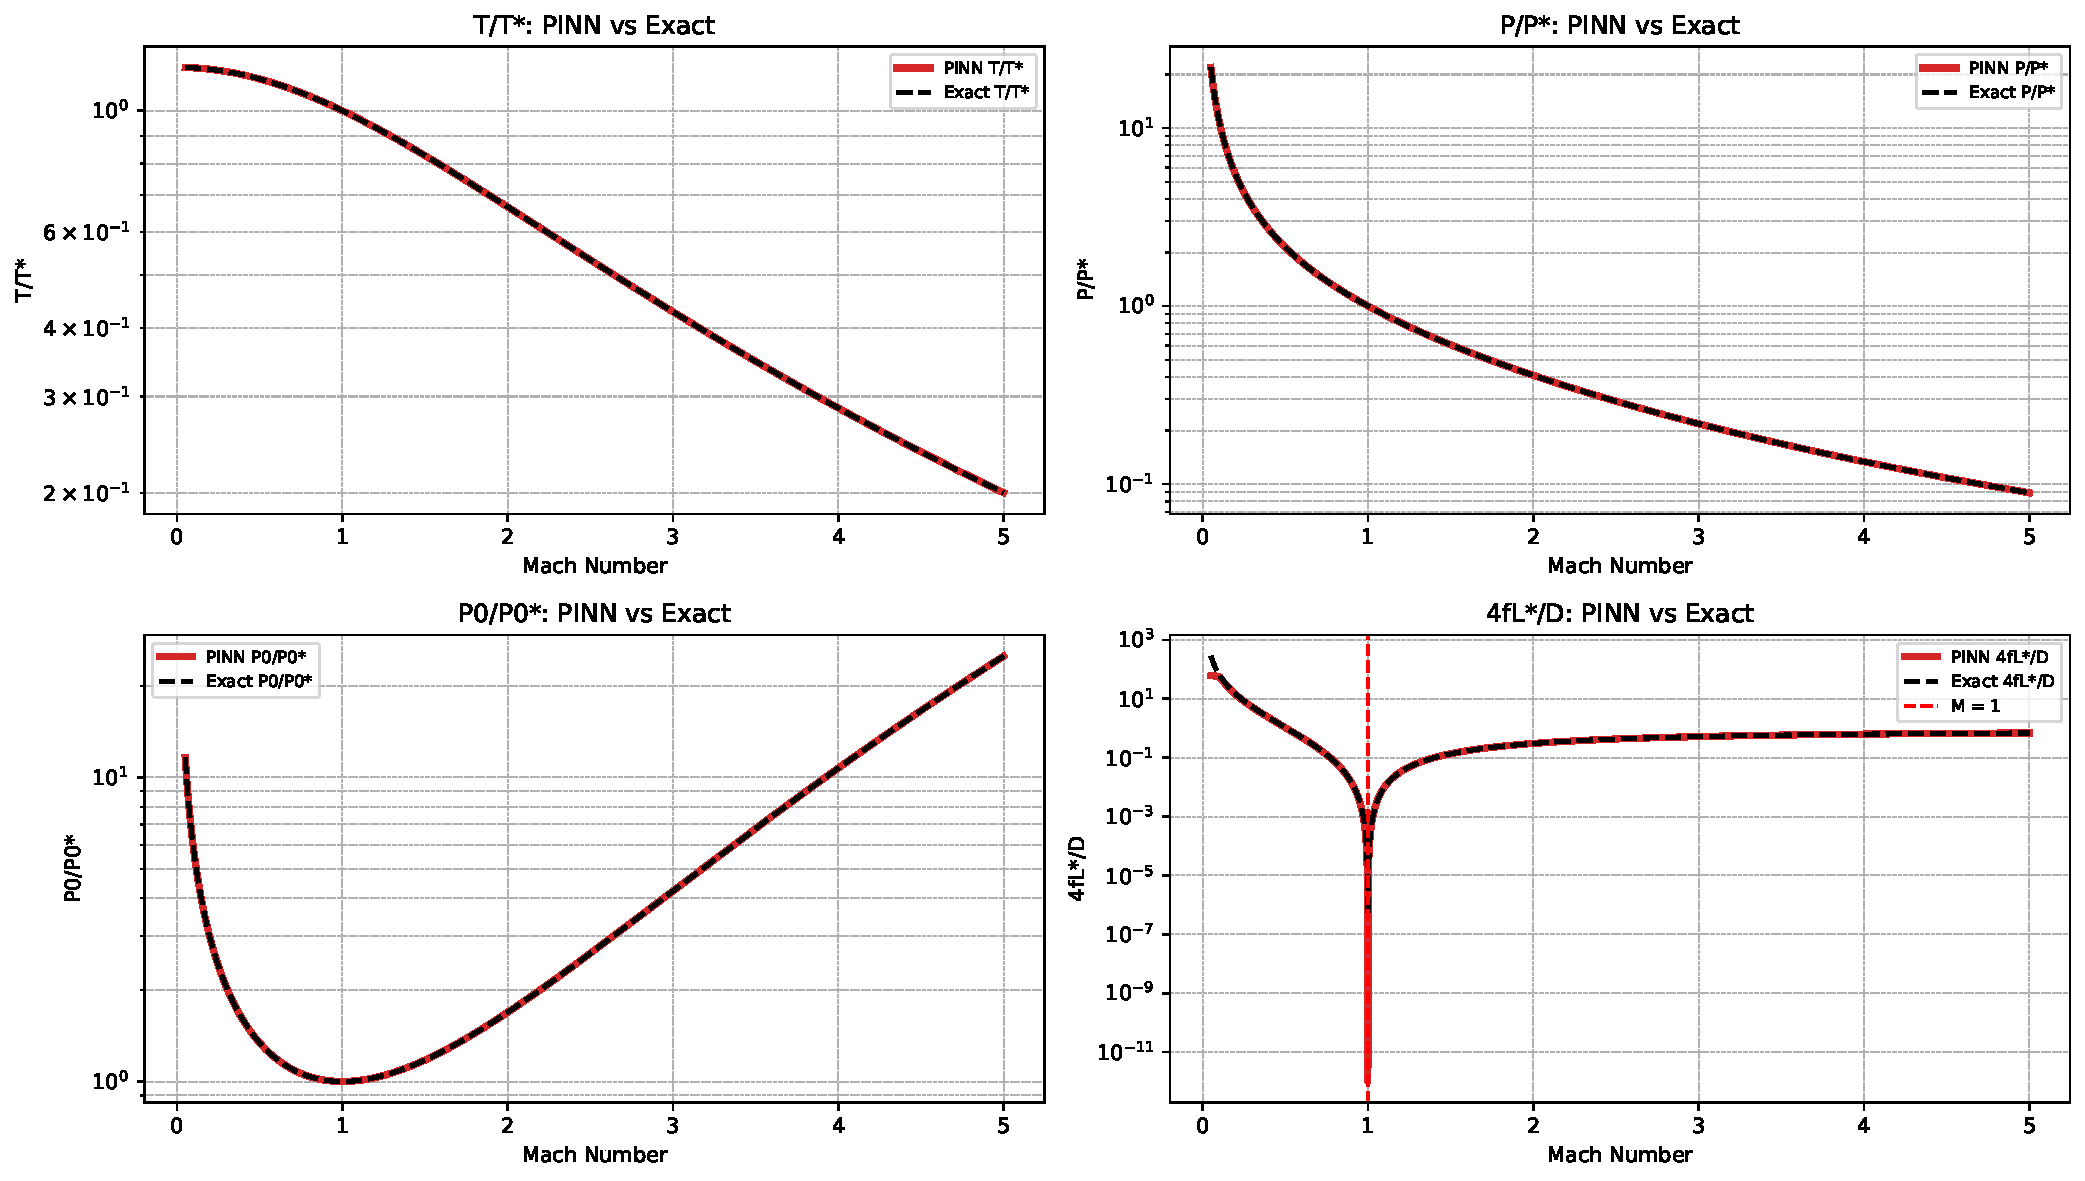
\includegraphics[width=0.95\textwidth]{fig_pinn_all_outputs.pdf}
\caption{Physics-Informed Neural Network (PINN) predictions (thick red lines) versus exact Fanno flow values (black dashed lines) for $T/T^*$, $P/P^*$, $P_0/P_0^*$, and $4fL^*/D$. The PINN learns $F(M) = 4fL^*/D$ by minimizing the ODE residual at collocation points; the auxiliary ratios $T/T^*$, $P/P^*$, and $P_0/P_0^*$ are reconstructed analytically from $M$. The vertical dashed line in the friction panel marks the sonic point.}
\label{fig:pinn_all_outputs}
\end{figure}

\paragraph{Relative Error Analysis}
Figure~\ref{fig:pinn_error} plots the relative error on $4fL^*/D$ alone. The temperature, pressure, and total-pressure ratios are omitted because they are reconstructed analytically from $M$ and therefore carry machine-zero error by construction; they are not network outputs and provide no PINN accuracy diagnostic.

\begin{figure}[h!]
\centering
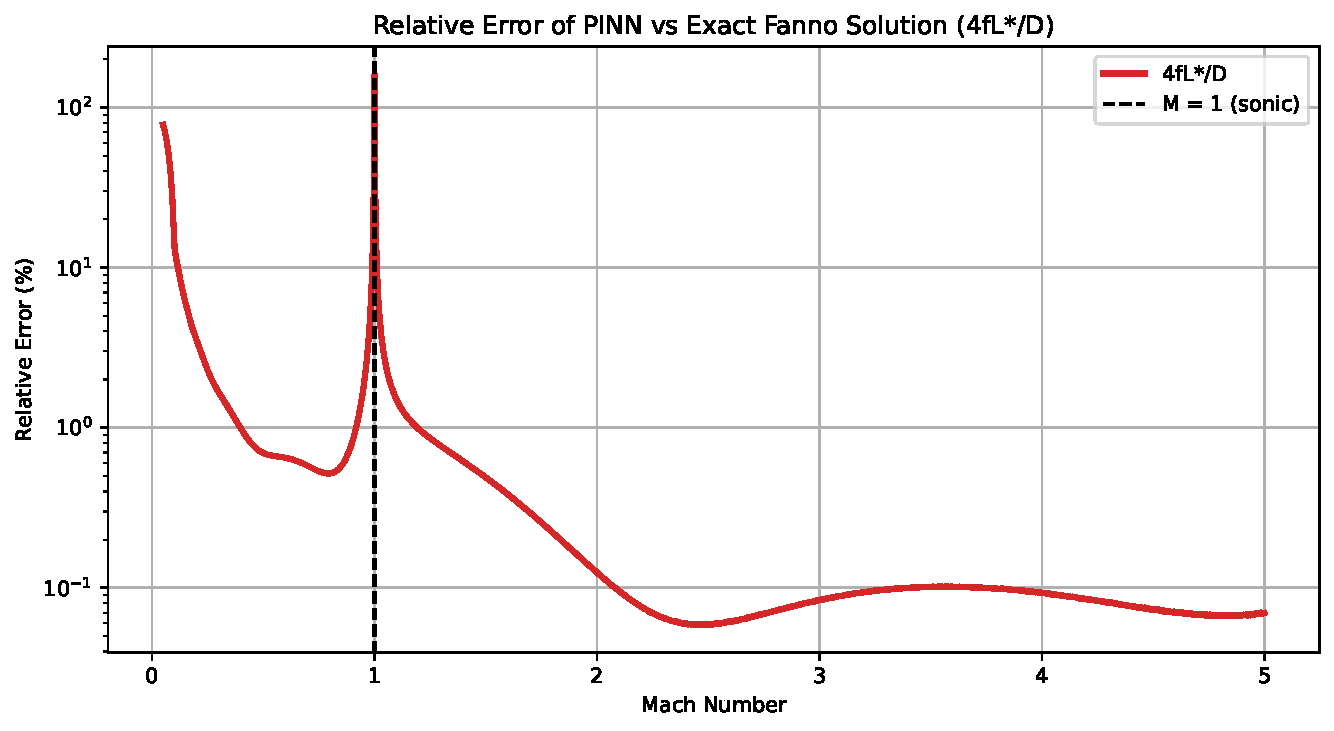
\includegraphics[width=0.85\textwidth]{fig_pinn_error.pdf}
\caption{Relative error (logarithmic scale) of the PINN-predicted friction parameter $4fL^*/D$ compared to the exact Fanno solution. Only $4fL^*/D$ is plotted because it is the sole learned output; $T/T^*$, $P/P^*$, and $P_0/P_0^*$ are analytical functions of $M$ and are exact by construction. The vertical dashed line indicates the sonic point ($M=1$), where $4fL^*/D$ vanishes and the relative error metric becomes ill-defined.}
\label{fig:pinn_error}
\end{figure}

\paragraph{Training Convergence}
The training history in Figure~\ref{fig:pinn_loss_history} shows the scaled ODE-residual loss decreasing as a function of epoch. Both the training curve and the validation curve use the same objective: the mean squared residual $(d\hat{F}/dM - \mathrm{RHS})/(|\mathrm{RHS}|+1)$ evaluated at collocation points during training and on a fixed dense grid over $M \in [0.1, 0.97] \cup [1.03, 5]$ during validation. The boundary condition does not appear in the loss because it is enforced by construction through the output transformation $\hat{F}(M) = (M-1)\,g_{\theta}(M)$. A smooth, near-monotonic decrease followed by a plateau indicates that the optimizer has converged to a low-residual solution; persistent plateaus or spikes typically signal that the learning-rate schedule, the number of collocation points, or the network capacity needs to be revisited.

\begin{figure}[h!]
\centering
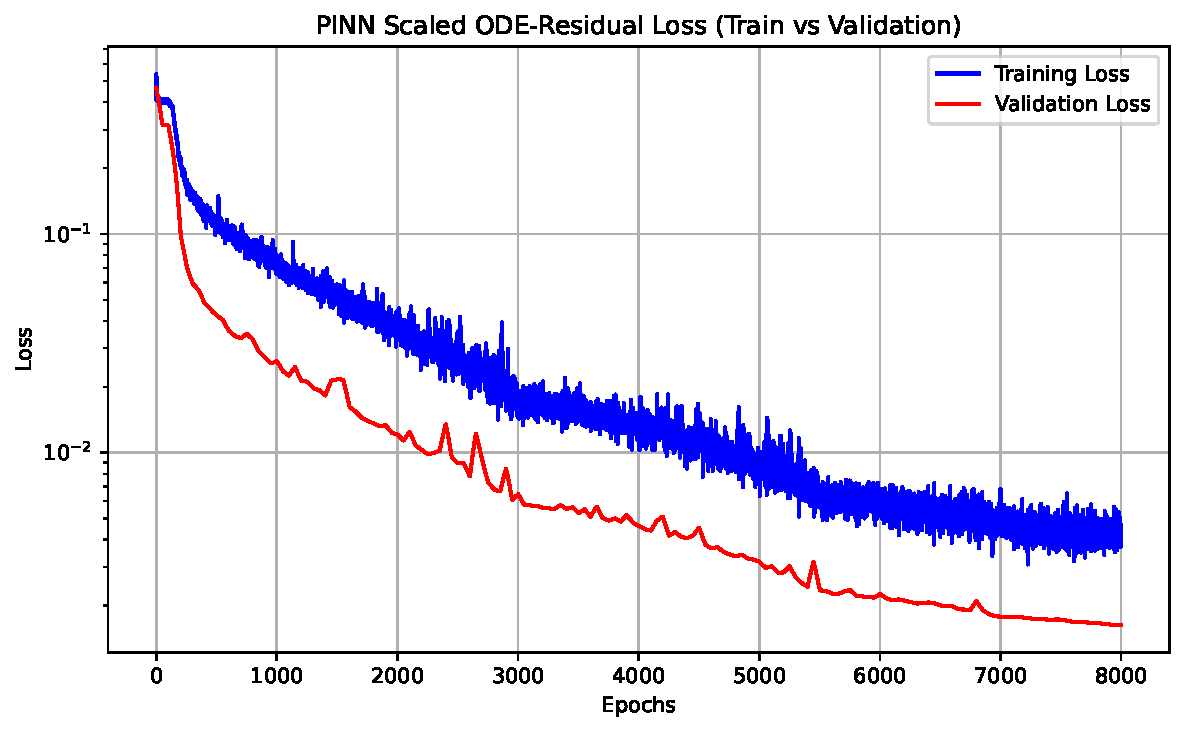
\includegraphics[width=0.7\textwidth]{fig_pinn_loss_history.pdf}
\caption{Physics-informed neural network training and validation loss versus epoch (logarithmic scale). Both curves report the scaled ODE residual of equation~\eqref{eq:pinn_loss}. Training loss is averaged over resampled collocation points each epoch; validation loss is the same residual evaluated on a fixed dense grid over $M \in [0.1, 0.97] \cup [1.03, 5]$. The two curves are directly comparable because they measure the same quantity.}
\label{fig:pinn_loss_history}
\end{figure}

\paragraph{Quantitative Validation}
Table~\ref{tab:mach_table_2} reports PINN predictions at representative Mach numbers spanning the subsonic, sonic, and supersonic regimes. The friction parameter $4 f L^{\ast}/D$ is the genuine PINN output: the relative error stays below $1.7\%$ across the entire domain, the worst case ($1.66\%$) occurring at $M = 0.3$ where the Fanno function is steepest, and the network reproduces the sonic anchor $F(1) = 0$ exactly by construction. The temperature and pressure ratios reported alongside it match the exact values to printed precision because they are reconstructed from analytical closed-form relations once $M$ is known. All of this is obtained using only the ODE residual, with no labelled $(M, F)$ pairs supplied during training.

\begin{table}[h!]
\centering
\small
\caption{PINN predictions versus exact Fanno values for $P_0/P_0^*$ and $4fL^*/D$. The friction parameter is the direct, learned output of the network and provides the meaningful accuracy diagnostic.}
\label{tab:mach_table_2}
\begin{tabular}{c|cc|cc}
\hline
$M$ & $P_0/P_0^*$ exact & $P_0/P_0^*$ PINN & $4fL^*/D$ exact & $4fL^*/D$ PINN \\
\hline
0.3 & 2.03507 & 2.03507 & 5.29925 & 5.21122 \\
0.6 & 1.18820 & 1.18820 & 0.49082 & 0.48763 \\
1.0 & 1.00000 & 1.00000 & 0.00000 & 0.00000 \\
1.5 & 1.17617 & 1.17617 & 0.13605 & 0.13672 \\
2.5 & 2.63672 & 2.63672 & 0.43198 & 0.43223 \\
3.0 & 4.23457 & 4.23457 & 0.52216 & 0.52260 \\
\hline
\end{tabular}
\end{table}

\paragraph{Educational Insights}
Three structural choices make the Fanno PINN succeed and transfer directly to more complex ODE and PDE problems in fluid dynamics. \textbf{Physics is the training signal:} the only loss term in equation~\eqref{eq:pinn_loss} is the ODE residual, so the network reconstructs the full Fanno function from the equation itself rather than from $(M,F)$ labels. \textbf{Hard boundary conditions are robust:} the transformation $\hat{F}(M) = (M-1)\,g_{\theta}(M)$ enforces $\hat{F}(1)=0$ to machine precision and eliminates one penalty term from the optimization. \textbf{Residual scaling balances stiff and smooth regions:} dividing the residual by $|\mathrm{RHS}|+1$, combined with log-uniform sampling on the subsonic branch, prevents the optimizer from chasing only the steep behaviour near $M\!\to\!0$ at the expense of the supersonic regime. The same workflow---network with hard BC, autodiff residual, scaled loss, and stratified collocation---generalizes directly to Rayleigh flow, nozzle flows, and unsteady wave propagation, where labelled data are typically expensive to obtain but the governing equations are well known.

\subsection{Comparison of the Three Approaches}
\label{sec:comparison}

Table~\ref{tab:method_comparison} consolidates the three approaches developed in this chapter against the criteria that matter most when selecting a model for a new gas-dynamics problem: what data are required, what physical guarantees the model carries by construction, the maximum relative error observed on the Fanno benchmark, the cost per query after training, and the principal failure mode of the method.

\begin{table}[h!]
\centering
\small
\caption{Comparison of polynomial Ridge regression, supervised surrogate neural network, and physics-informed neural network on the Fanno flow benchmark with $\gamma = 1.4$, $M \in [0.05, 5.0]$.}
\label{tab:method_comparison}
\begin{tabular}{p{3.0cm} p{3.1cm} p{3.1cm} p{3.1cm}}
\toprule
\textbf{Criterion} & \textbf{Poly-Ridge regression} & \textbf{Supervised surrogate NN} & \textbf{Physics-informed NN} \\
\midrule
Training data & $\sim\!10^{4}$ labelled $(M,\mathbf{y})$ pairs & $\sim\!10^{4}$ labelled $(M,\mathbf{y})$ pairs & none (only the ODE and BC) \\
Physics enforced? & no, only via engineered features & no & yes, by ODE residual and hard BC \\
Validation MAE on $4fL^{*}/D$ & $\sim\!3\!\times\!10^{-5}$ & $\sim\!10^{-3}$ & $\sim\!10^{-2}$ \\
Generalization outside training data & poor (extrapolation drifts) & poor (no structural law) & good (governed by the ODE) \\
Cost per query & forward eval of polynomial & one network forward pass & one network forward pass + closed-form auxiliaries \\
Differentiability & analytic & autodiff & autodiff (used during training) \\
Principal failure mode & feature engineering breaks down for unknown physics & violates conservation laws far from data & non-convex loss; sensitive to sampling and weighting \\
Best use case & known closed-form structure, abundant data & high-dimensional parameter sweeps, real-time evaluation & sparse/noisy data, known governing equations \\
\bottomrule
\end{tabular}
\end{table}

The three methods are not strictly ordered: each owns a region of problem space. Where the analytical structure of the equations is fully known and labelled data are abundant, polynomial Ridge regression with engineered features is the cheapest and most accurate choice. Where the parameter space is large and many forward evaluations are required, a supervised surrogate trained on cached solver runs is the appropriate accelerator. Where the governing equations are known but data are sparse, expensive, or contaminated by measurement noise---the typical industrial situation---PINNs are the only one of the three that retains physical consistency in the data-poor regions of the domain.

\subsection{Limitations and Common Pitfalls}
\label{sec:pitfalls}

The Fanno benchmark is well behaved, and all three methods reach engineering accuracy. Practitioners who carry the same workflow to less forgiving problems should keep four recurring pitfalls in mind. \textbf{Spurious extrapolation} is the dominant failure mode of regression and supervised surrogates, both of which can produce smooth-looking but unphysical predictions outside the training distribution \cite{Brunton2020}; an explicit envelope of validity is therefore mandatory. \textbf{Non-convex PINN training} is sensitive to loss weighting, learning-rate schedule, and collocation distribution \cite{Urban2025,Cuomo2022}; remedies include residual scaling (used here), adaptive weights, curriculum learning, and domain decomposition \cite{Jagtap2020,Kharazmi2021}. \textbf{Stiff regions and singularities} (here $\mathrm{RHS}(M)\!\sim\!1/M^{3}$ near $M\!\to\!0$ and the removable singularity at $M\!=\!1$) demand stratified sampling, hard-BC transforms, or weak-form formulations \cite{Kharazmi2021,Lu2021hPINN}. \textbf{Smooth activations} such as $\tanh$ or Swish \cite{Ramachandran2017} are required because PINNs differentiate the network analytically and ReLU destroys the residual computation. These caveats are not a critique of AI methods; they are the operational checklist that distinguishes a research demonstration from a deployable engineering surrogate.

\subsection{Summary and Perspective}

This chapter has built a hierarchy of AI methods on top of a single, well-controlled gas-dynamics benchmark. Each step of the hierarchy adds one ingredient and removes one limitation:

\begin{enumerate}
    \item \textbf{Polynomial Ridge regression} with physics-engineered features ($M$, $M^{2}$, $1/M$, $1/M^{2}$, $\ln M$) reproduces the four Fanno outputs with $R^{2}\!\approx\!1$ and validation MAE on the order of $10^{-5}$. The lesson is that, when the analytical structure of the governing equations is known, embedding it directly into the input space converts a strongly nonlinear problem into a near-linear one.
    \item \textbf{Forward surrogate neural networks} extend this capability without requiring a hand-derived feature set. They provide smooth, multi-output approximations that generalize across the entire Mach domain and cost a single forward pass per query, making them well suited for parametric design studies or real-time applications. They remain, however, purely data-driven: outside the training distribution they have no structural reason to obey conservation laws.
    \item \textbf{Physics-informed neural networks} restore that structural reason. By replacing the supervised loss with the ODE residual computed via automatic differentiation, the network is constrained to satisfy the Fanno equation everywhere it is evaluated, even at points where no labelled data are available. With a hard sonic boundary condition $\hat{F}(M) = (M-1)\,g_{\theta}(M)$ and a residual rescaled by $1/(|\mathrm{RHS}|+1)$, the network reproduces the cumulative friction parameter to within a few percent across $M \in [0.1, 5]$ using \emph{no} labelled $(M, F)$ pairs.
\end{enumerate}

The progression from regression to surrogate to PINN is not a ranking but a spectrum: each method occupies its own niche. Regression and surrogate networks are appropriate when training data are abundant and the governing equations are unknown or uncertain; PINNs are appropriate when the equations are known but data are scarce, expensive, or noisy. Hybrid formulations that combine both signals (data anchors plus ODE residual) are common in practice and were discussed in passing.

Although the Fanno hierarchy focused on a steady, one-dimensional ODE, the same workflow---hierarchical model selection, physics-informed feature design, autodiff residuals, and hard boundary-condition transformations---applies directly to Rayleigh flow, nozzle flows, oblique-shock relations, and unsteady wave propagation. Fanno flow is therefore a pedagogical bridge: simple enough to admit an analytical reference, rich enough to expose every difficulty (stiffness near $M\!\to\!0$, a singular sonic point, multi-scale outputs) that practitioners will face when extending these methods to engineering problems where no closed-form solution exists.

The Burgers section that follows extends the chapter to the second pillar of shock-wave dynamics. Where Fanno isolated a singular sonic point inside a steady scalar ODE and rewarded a hard boundary-condition transformation, Burgers isolates a spontaneously forming viscous layer inside an unsteady scalar PDE and rewards a soft penalty formulation against the Cole--Hopf analytical reference. The PINN workflow itself is essentially unchanged: a smooth-activation network, an automatic-differentiation residual, scaled or weighted loss terms, and a stratified collocation strategy. What changes is the input dimension (from $M$ to $(x,t)$), the number of derivatives the residual requires (one to three), and the way the boundary and initial conditions are imposed (hard transformation versus soft penalty). Read together, Fanno and Burgers cover the two structural difficulties---singularities of the governing equation and discontinuities of its solution---that practitioners will face when carrying these techniques forward to the Sod shock-tube problem and to multidimensional compressible flows.

\section{Burgers' Equation}

\subsection{Introduction and Physical Intuition}

Fanno flow provided a steady, one-dimensional benchmark with a sonic singularity but no genuine discontinuity. Real gas-dynamics applications routinely involve unsteady waves that steepen into shocks; capturing this behaviour is the next test of any AI-based methodology. Burgers' equation \cite{Burgers1948} is the simplest model that retains the essential mechanism of shock formation in compressible flow: the nonlinear advection term $u\,\partial_x u$ steepens any compressive disturbance, while a small viscous term $\nu\,\partial_{xx} u$ counteracts the steepening through molecular diffusion. The resulting balance produces a thin internal layer that mimics the structure of a viscous shock wave \cite{Whitham1974}.

In its inviscid form, Burgers' equation is

\begin{equation}
\label{eq:burgers_inviscid}
\frac{\partial u}{\partial t} \;+\; u\,\frac{\partial u}{\partial x} \;=\; 0,
\end{equation}

a hyperbolic conservation law whose characteristics carry the value of $u$ along trajectories of slope $u$ in the $(x,t)$ plane. Compressive initial data therefore generate intersecting characteristics in finite time, beyond which the classical solution ceases to exist and a discontinuity must be admitted. The Rankine--Hugoniot jump condition $s = (u_L + u_R)/2$ relates the shock speed $s$ to the states on either side and selects the unique entropy-satisfying weak solution \cite{LeVeque2002}.

The viscous form,

\begin{equation}
\label{eq:burgers_viscous}
\frac{\partial u}{\partial t} \;+\; u\,\frac{\partial u}{\partial x} \;=\; \nu\,\frac{\partial^{2} u}{\partial x^{2}},
\end{equation}

regularizes the inviscid limit by adding a diffusion term of strength $\nu \ge 0$. For $\nu \to 0$ the viscous solution converges to the entropy-admissible weak solution of equation~\eqref{eq:burgers_inviscid}; for finite $\nu$ the solution is smooth everywhere, with shock-like layers of thickness proportional to $\nu/\Delta u$.

Burgers' equation occupies a precise position in the gas-dynamics hierarchy. Starting from the one-dimensional Euler system that governs the shock tube, dropping the pressure work and the energy equation, and retaining only the nonlinear momentum advection produces a scalar conservation law whose viscous regularization is exactly equation~\eqref{eq:burgers_viscous}. Burgers is therefore the scalar precursor to the full Euler shock-tube problem. From the AI perspective, Fanno gives us a steady ODE in $M$; Burgers gives us an unsteady, one-dimensional PDE with a forming discontinuity; the shock tube is the natural next step in the chain.

The remainder of this section presents two complementary PINN demonstrations driven by the same compressive sinusoidal initial condition $u(x, 0) = -\sin(\pi x)$ on $[-1, 1]$ with zero Dirichlet boundary data. The first demonstration takes the inviscid form (equation~\eqref{eq:burgers_inviscid}) on the pre-breaking time horizon $t \in [0, 0.30]$ and uses the implicit characteristic equation as the analytical reference. The second demonstration takes the viscous form (equation~\eqref{eq:burgers_viscous}) on the full window $t \in [0, 1]$ with $\nu = 0.01/\pi$, the canonical configuration of Raissi, Perdikaris, and Karniadakis~\cite{Raissi2019PINN} that has become the de-facto benchmark for PINN methods on Burgers' equation. Both demonstrations use independent TensorFlow~2 implementations with an eight- or six-layer $\tanh$ MLP architecture, an Adam pretraining stage, and an L-BFGS-B refinement stage on the flattened weight vector.

\subsection{Inviscid Burgers PINN: Pre-Breaking Demonstration}
\label{sec:burgers_inviscid_demo}

The inviscid initial-value problem
\[
u_{t} + u\,u_{x} = 0,
\qquad u(x, 0) = -\sin(\pi x),
\qquad u(\pm 1, t) = 0,
\]
admits an exact solution by the method of characteristics for $t < t^{*}_{\mathrm{break}} = 1/\pi$. Each characteristic is the line $x(t) = x_{0} + u(x_{0}, 0)\,t = x_{0} - \sin(\pi x_{0})\,t$ in the $(x, t)$-plane, along which the value of $u$ is preserved. The map $x_{0} \mapsto x_{0} - \sin(\pi x_{0})\,t$ is invertible for $t < 1/\pi$, so the solution at any $(x, t)$ in the pre-breaking window is recovered by solving the implicit equation $x = x_{0} - \sin(\pi x_{0})\,t$ for $x_{0}$ and setting $u(x, t) = -\sin(\pi x_{0})$. We solve this implicit equation by vectorised Newton iteration; the result is exact to machine precision and provides the analytical anchor for the inviscid PINN. Beyond $t = 1/\pi$ the solution acquires a stationary shock at $x = 0$ that the smooth network cannot represent without modification, so we restrict the inviscid demonstration to $t \in [0, 0.30]$.

\paragraph{Network and Loss}
The inviscid PINN is a six-layer $\tanh$ MLP with $20$ neurons per layer (smaller than the viscous network because the residual contains only first derivatives). Inputs are $(x, t)$, normalised to $[-1, 1]$ before entering the first hidden layer; the output is a single scalar $u_{\theta}(x, t)$. The loss is

\begin{equation}
\label{eq:burgers_inv_loss}
\mathcal{L}_{\mathrm{inv}} \;=\; \frac{1}{N_{f}}\sum_{i=1}^{N_{f}}
\!\left[ \partial_{t} u_{\theta} + u_{\theta}\,\partial_{x} u_{\theta} \right]^{2}_{(x_{i}^{f}, t_{i}^{f})}
\;+\; \mathcal{L}_{\mathrm{IC}}
\;+\; \mathcal{L}_{\mathrm{BC}},
\end{equation}

with the same soft initial- and boundary-condition penalties used for the viscous case. Eight thousand interior collocation points are drawn uniformly in $[-1, 1] \times [0, 0.30]$, $200$ points sample the initial line $t = 0$, and $200$ points sample the lateral boundaries $x = \pm 1$. Training applies $2{,}000$ Adam epochs at learning rate $10^{-3}$, then up to $800$ L-BFGS-B iterations.

\paragraph{Results}
Figure~\ref{fig:burgers_inviscid_snapshots} shows three snapshots of $u_{\theta}(x, t^{*})$ at $t^{*} = 0.10$, $0.20$, $0.28$ together with the characteristic-based exact solution. The compressive ridge near $x = 0$ steepens monotonically as $t \to 1/\pi$; the PINN tracks the steepening profile with peak pointwise error below $7\%$ even at $t = 0.28$, where the slope $\partial_{x} u$ at $x = 0$ is approaching infinity. Figure~\ref{fig:burgers_inviscid_contour} displays the predicted space--time field over the entire training horizon and confirms that the network reproduces the inflection-point migration along the line $x = 0$ without spurious oscillations. Quantitative errors are reported in Table~\ref{tab:burgers_inviscid_errors}.

\begin{figure}[h!]
\centering
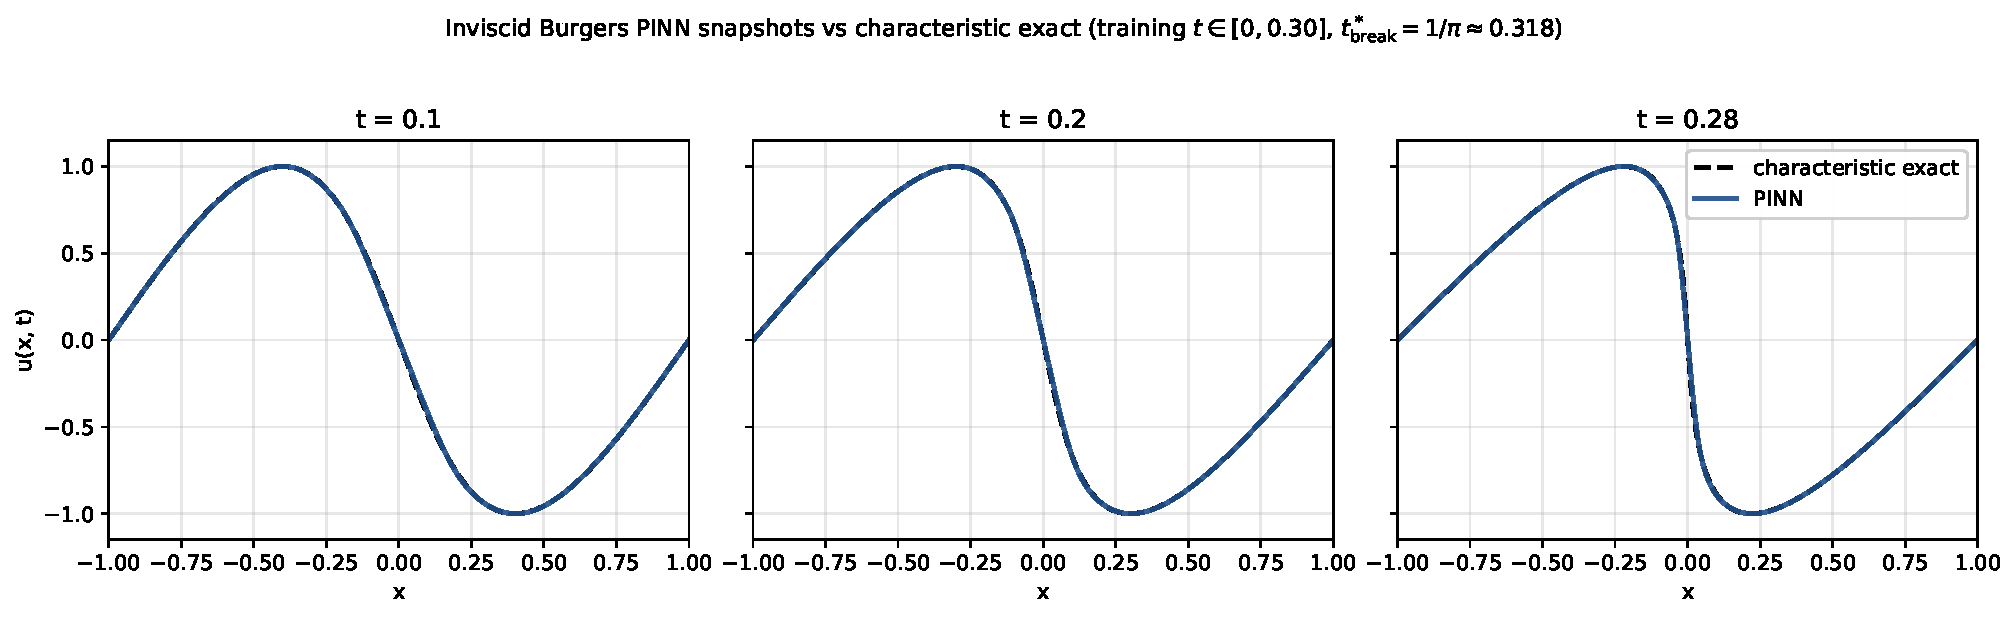
\includegraphics[width=0.95\textwidth]{fig_burgers_inviscid_snapshots.pdf}
\caption{Inviscid Burgers PINN snapshot comparison at $t^{*} = 0.10$, $0.20$, $0.28$. Thick blue lines show the PINN prediction $u_{\theta}(x, t^{*})$; black dashed lines show the exact characteristic solution obtained by Newton inversion of $x = x_{0} - \sin(\pi x_{0})\,t$. The classical breaking time $t^{*}_{\mathrm{break}} = 1/\pi \approx 0.318$ is approached but not crossed; the slope at $x = 0$ tightens steadily and the PINN tracks it without numerical oscillation.}
\label{fig:burgers_inviscid_snapshots}
\end{figure}

\begin{figure}[h!]
\centering
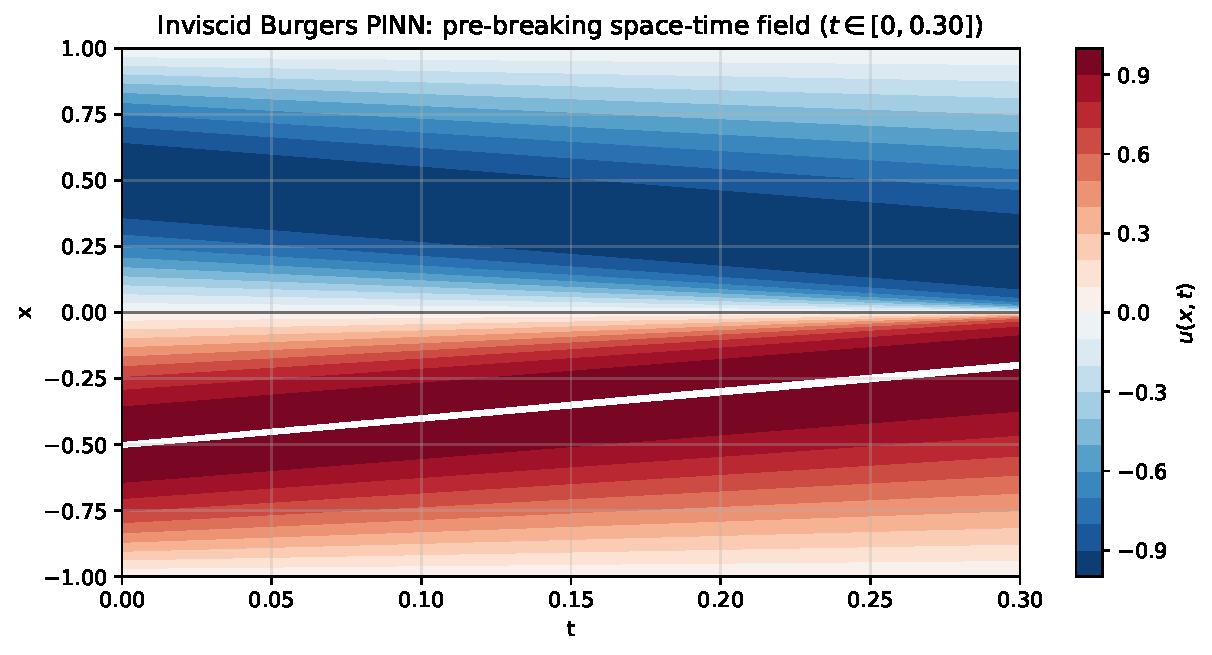
\includegraphics[width=0.85\textwidth]{fig_burgers_inviscid_contour.pdf}
\caption{Inviscid Burgers PINN: predicted velocity $u_{\theta}(x, t)$ over the pre-breaking horizon $t \in [0, 0.30]$. The compressive characteristic family converging on $x = 0$ is clearly visible; for $t > 1/\pi$ characteristics would cross and the smooth network solution would no longer be admissible.}
\label{fig:burgers_inviscid_contour}
\end{figure}

\begin{table}[h!]
\centering
\small
\caption{Inviscid Burgers PINN snapshot accuracy. The relative $L_{2}$ error is $\|u_{\theta}(\cdot, t^{*}) - u_{\mathrm{char}}(\cdot, t^{*})\|_{2} / \|u_{\mathrm{char}}(\cdot, t^{*})\|_{2}$, evaluated on a uniform grid of $401$ points in $x \in [-1, 1]$. Error grows monotonically with $t^{*}$, in line with the diverging slope of the characteristic solution as $t \to 1/\pi$.}
\label{tab:burgers_inviscid_errors}
\begin{tabular}{c c c}
\toprule
$t^{*}$ & Relative $L_{2}$ error & Peak pointwise error \\
\midrule
$0.10$ & $6.22 \times 10^{-3}$ & $1.73 \times 10^{-2}$ \\
$0.20$ & $7.93 \times 10^{-3}$ & $2.85 \times 10^{-2}$ \\
$0.28$ & $1.21 \times 10^{-2}$ & $6.93 \times 10^{-2}$ \\
\bottomrule
\end{tabular}
\end{table}

The inviscid demonstration also illustrates a fundamental limitation of standard PINNs. The characteristic solution becomes multi-valued for $t > 1/\pi$ and must be replaced by an entropy-admissible weak solution containing a stationary shock at $x = 0$. A smooth $\tanh$ network cannot represent a true discontinuity; pushing the training horizon past the breaking time without an additional regularisation mechanism (added artificial viscosity, weak-form residual, or domain decomposition with internal Rankine--Hugoniot constraints) produces a smooth ramp instead of a shock, with the wrong propagation speed and an unphysically smeared profile. Adding a small viscosity, as in the next subsection, is the simplest and most widely used such regularisation.

\subsection{Viscous Burgers PINN: Raissi Benchmark}
\label{sec:burgers_reference}

The second demonstration adopts the canonical benchmark introduced by Raissi, Perdikaris, and Karniadakis~\cite{Raissi2019PINN}, who used it to establish PINNs as a method for nonlinear PDE regression. The configuration

\begin{equation}
\label{eq:burgers_setup}
\begin{aligned}
&\frac{\partial u}{\partial t} + u\,\frac{\partial u}{\partial x} \;=\; \nu\,\frac{\partial^{2} u}{\partial x^{2}},
&& (x, t) \in [-1, 1] \times [0, 1], \\[0.5ex]
&u(x, 0) \;=\; -\sin(\pi x),
&& \text{initial condition}, \\[0.5ex]
&u(-1, t) \;=\; u(1, t) \;=\; 0,
&& \text{Dirichlet boundary conditions}, \\[0.5ex]
&\nu \;=\; 0.01/\pi,
&& \text{kinematic viscosity},
\end{aligned}
\end{equation}

is used unchanged here. The smooth sinusoidal initial condition is compressive near $x = 0$, where $\partial_{x} u < 0$ for $|x| < 1/2$, as discussed in the inviscid demonstration; for the chosen viscosity the smooth profile rapidly transitions into a thin internal layer centred on $x = 0$ shortly after $t = 1/\pi$, and that layer persists until the end of the integration window. Crucially, the viscosity removes the discontinuity that defeated the inviscid PINN beyond the breaking time: the solution is smooth for all $t \ge 0$, and a $\tanh$ network can represent it.

The viscous Burgers equation admits an exact solution through the Cole--Hopf transformation \cite{Cole1951, Hopf1950}. Substituting $u = -2\nu\,\partial_x \phi / \phi$ converts equation~\eqref{eq:burgers_viscous} into the linear heat equation $\partial_t \phi = \nu\,\partial_{xx}\phi$, which can be solved by superposition of Gaussian kernels for the initial condition $\phi(x, 0) = \exp\!\left[-(2\nu)^{-1}\int_{0}^{x} u(\xi, 0)\,d\xi\right]$. The reference solution $u_{\mathrm{exact}}(x, t)$ used throughout this section is computed by Gauss--Hermite quadrature of the resulting Cole--Hopf integral on a fine $(x, t)$ grid; it is exact to machine precision modulo quadrature error, and serves as the analytical anchor for the viscous PINN comparison.

\paragraph{Network Architecture}
The viscous PINN is a fully connected feedforward network $u_{\theta}(x, t)$ with the following structure:

\begin{itemize}
    \item \textbf{Input.} Two scalars $(x, t)$. Both are normalized to $[-1, 1]$ before entering the first hidden layer to keep the activation regime well conditioned.
    \item \textbf{Hidden layers.} Eight fully connected layers of $20$ neurons each, with $\tanh$ activations \cite{Goodfellow2016}, following the reference configuration \cite{Raissi2019PINN}. The smooth differentiability of $\tanh$ is essential because automatic differentiation must produce three accurate derivatives ($u_t$, $u_x$, $u_{xx}$) at every collocation point.
    \item \textbf{Output.} A single linear neuron returns $u_{\theta}(x, t)$. Unlike the Fanno PINN, the boundary and initial conditions are imposed as soft penalties rather than baked into an output transformation, because the conditions are distributed along three distinct manifolds of $\partial \Omega \times [0,T] \cup \Omega \times \{0\}$ rather than at a single point. A short note on hard-IC/BC alternatives, such as transformations of the form $u_{\theta}(x,t) = (1-x^{2})\,t\,g_{\theta}(x,t) + (1-t)\,(-\sin\pi x)$, is given in the educational insights below.
\end{itemize}

\paragraph{Loss Function}
The composite loss combines a PDE-residual term, an initial-condition term, and a boundary-condition term:

\begin{equation}
\label{eq:burgers_loss}
\mathcal{L}_{\mathrm{PINN}} \;=\; \mathcal{L}_{\mathrm{PDE}} \;+\; \lambda_{\mathrm{IC}}\,\mathcal{L}_{\mathrm{IC}} \;+\; \lambda_{\mathrm{BC}}\,\mathcal{L}_{\mathrm{BC}},
\end{equation}

with the three contributions defined as

\begin{equation}
\label{eq:burgers_components}
\begin{aligned}
\mathcal{L}_{\mathrm{PDE}} &\;=\; \frac{1}{N_{f}} \sum_{i=1}^{N_{f}}
\left[
\frac{\partial u_{\theta}}{\partial t}(x_{i}^{f}, t_{i}^{f}) \;+\; u_{\theta}\,\frac{\partial u_{\theta}}{\partial x}(x_{i}^{f}, t_{i}^{f}) \;-\; \nu\,\frac{\partial^{2} u_{\theta}}{\partial x^{2}}(x_{i}^{f}, t_{i}^{f})
\right]^{2}, \\[1ex]
\mathcal{L}_{\mathrm{IC}} &\;=\; \frac{1}{N_{0}} \sum_{j=1}^{N_{0}}
\left[ u_{\theta}(x_{j}^{0}, 0) \;+\; \sin(\pi x_{j}^{0}) \right]^{2}, \\[1ex]
\mathcal{L}_{\mathrm{BC}} &\;=\; \frac{1}{N_{b}} \sum_{k=1}^{N_{b}}
\left[ u_{\theta}(-1, t_{k}^{b})^{2} \;+\; u_{\theta}(1, t_{k}^{b})^{2} \right].
\end{aligned}
\end{equation}

The collocation sets $\{(x_{i}^{f}, t_{i}^{f})\}$, $\{x_{j}^{0}\}$, and $\{t_{k}^{b}\}$ are sampled at the start of training: $N_{f} = 10{,}000$ interior points drawn uniformly in $\Omega \times [0,T]$, $N_{0} = 200$ initial-condition points uniform in $x$, and $N_{b} = 200$ boundary points uniform in $t$. The weights $\lambda_{\mathrm{IC}}$ and $\lambda_{\mathrm{BC}}$ are set so that the three terms remain commensurate at initialization; in practice, $\lambda_{\mathrm{IC}} = \lambda_{\mathrm{BC}} = 1$ is sufficient when $N_{f}/N_{0} = N_{f}/N_{b} \approx 50$, because the per-point IC and BC residuals are larger than the unscaled PDE residual at start of training.

\paragraph{Training Procedure}
Training follows the two-stage protocol that has become standard for PINN regression on Burgers-type problems \cite{Raissi2019PINN}. A first stage of $3{,}000$ Adam epochs \cite{Kingma2015Adam} with learning rate $10^{-3}$ provides rapid descent to a moderate-residual solution. A second stage of L-BFGS \cite{LiuNocedal1989} (up to $1{,}200$ quasi-Newton iterations) is then applied to refine the network into the high-accuracy basin where the residual is dominated by the shock layer. Each Adam step performs a forward pass on $(x_{i}^{f}, t_{i}^{f})$, computes $\partial_{t} u$, $\partial_{x} u$, and $\partial_{xx} u$ via nested gradient tapes, evaluates equations~\eqref{eq:burgers_loss}--\eqref{eq:burgers_components}, and backpropagates to the network parameters.

The collocation distribution can also be made adaptive: residual-based resampling concentrates points near the shock layer once the profile begins to steepen, accelerating convergence on the most informative region of $(x, t)$-space \cite{Lu2021hPINN}. We retain the uniform sampling of the original configuration to keep the comparison clean, but flag adaptive sampling as the natural upgrade for problems with stronger or moving shocks.

\paragraph{Results}

Figure~\ref{fig:burgers_snapshots} compares PINN snapshots $u_{\theta}(x, t^{*})$ with the Cole--Hopf reference at three representative times $t^{*} = 0.25$, $0.5$, $0.75$, spanning the smooth-profile, just-after-breaking, and post-formation regimes. The PINN reproduces the steepening sinusoid before $t^{*} = t^{*}_{\mathrm{break}}$ and resolves the thin internal layer that develops thereafter. Figure~\ref{fig:burgers_contour} shows the full space--time field $u_{\theta}(x, t)$ as a contour plot, with the steep-gradient ridge along the line $x = 0$ clearly visible for $t \gtrsim 0.32$. Figure~\ref{fig:burgers_loss_history} reports the loss history during the Adam stage; the L-BFGS refinement that follows reduces the loss by an additional one to two orders of magnitude in a small number of additional iterations.

\begin{figure}[h!]
\centering
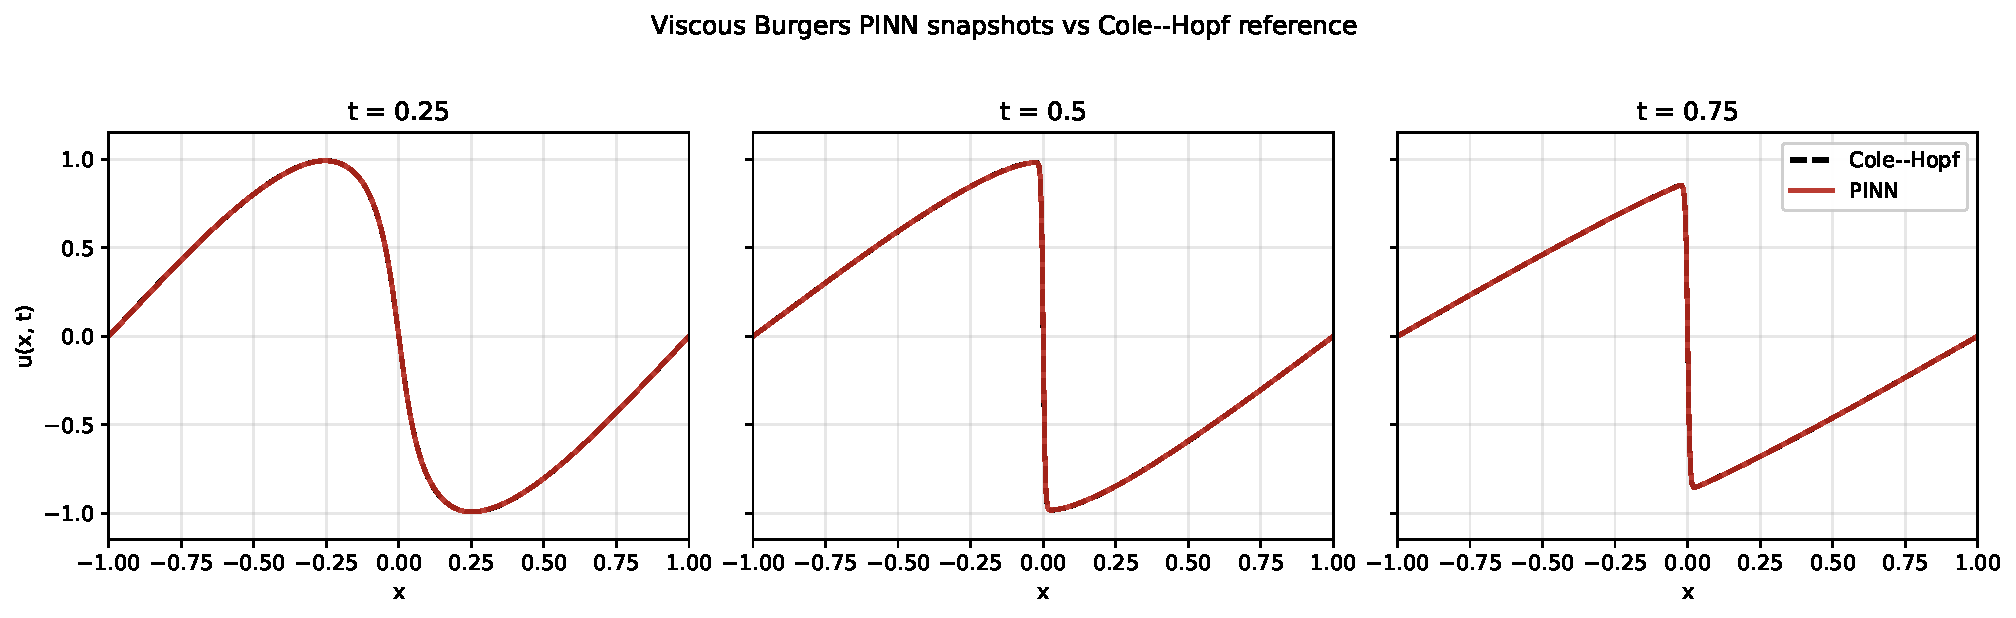
\includegraphics[width=0.95\textwidth]{fig_burgers_snapshots.pdf}
\caption{Burgers PINN snapshot comparison at $t^{*} = 0.25$, $0.5$, $0.75$. Thick red lines show the PINN prediction $u_{\theta}(x, t^{*})$; black dashed lines show the Cole--Hopf reference. The compressive sinusoid steepens during the smooth-profile phase ($t^{*} = 0.25$), develops a thin internal layer just after the classical breaking time $t^{*}_{\mathrm{break}} = 1/\pi$ (snapshot at $t^{*} = 0.5$), and persists with mild diffusive thickening at later times ($t^{*} = 0.75$). The viscosity is $\nu = 0.01/\pi$.}
\label{fig:burgers_snapshots}
\end{figure}

\begin{figure}[h!]
\centering
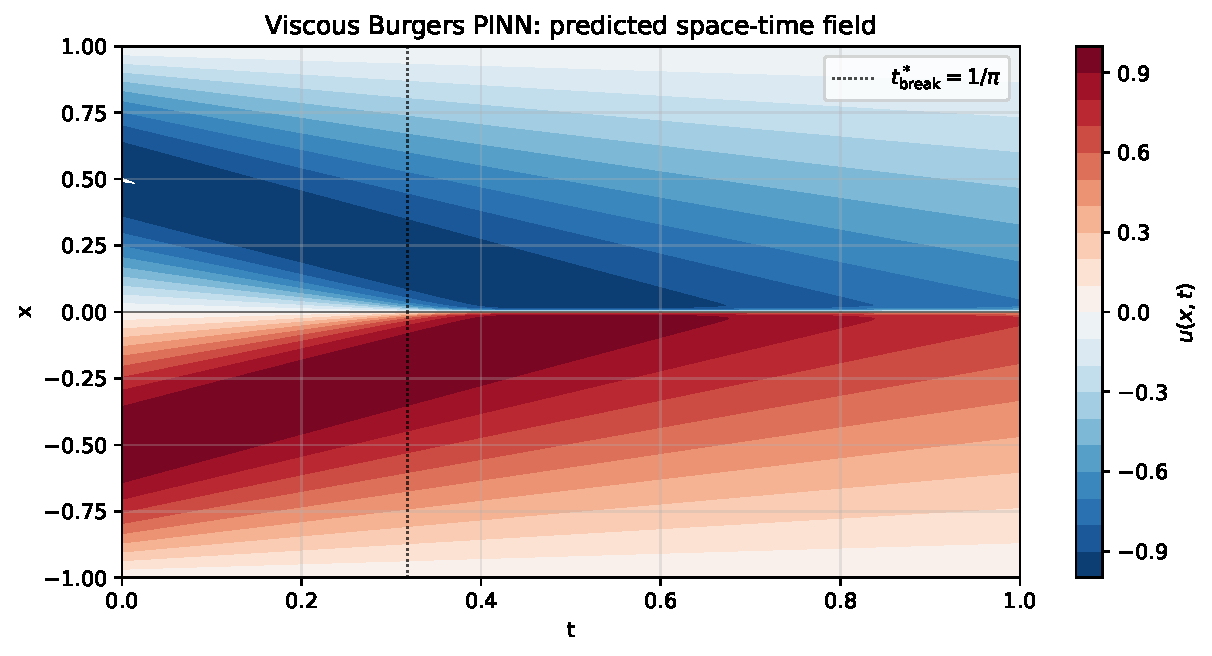
\includegraphics[width=0.85\textwidth]{fig_burgers_contour.pdf}
\caption{Space--time contour plot of the PINN-predicted velocity $u_{\theta}(x, t)$ for the Burgers benchmark. The compressive ridge $\partial_{x} u < 0$ near $x = 0$ tightens as $t$ approaches the classical breaking time $t^{*}_{\mathrm{break}} = 1/\pi \approx 0.318$ and persists as a thin viscous layer thereafter. Boundary values $u(-1, t) = u(1, t) = 0$ and the initial profile $u(x, 0) = -\sin(\pi x)$ are reproduced by the soft IC and BC penalties of equation~\eqref{eq:burgers_components}.}
\label{fig:burgers_contour}
\end{figure}

\begin{figure}[h!]
\centering
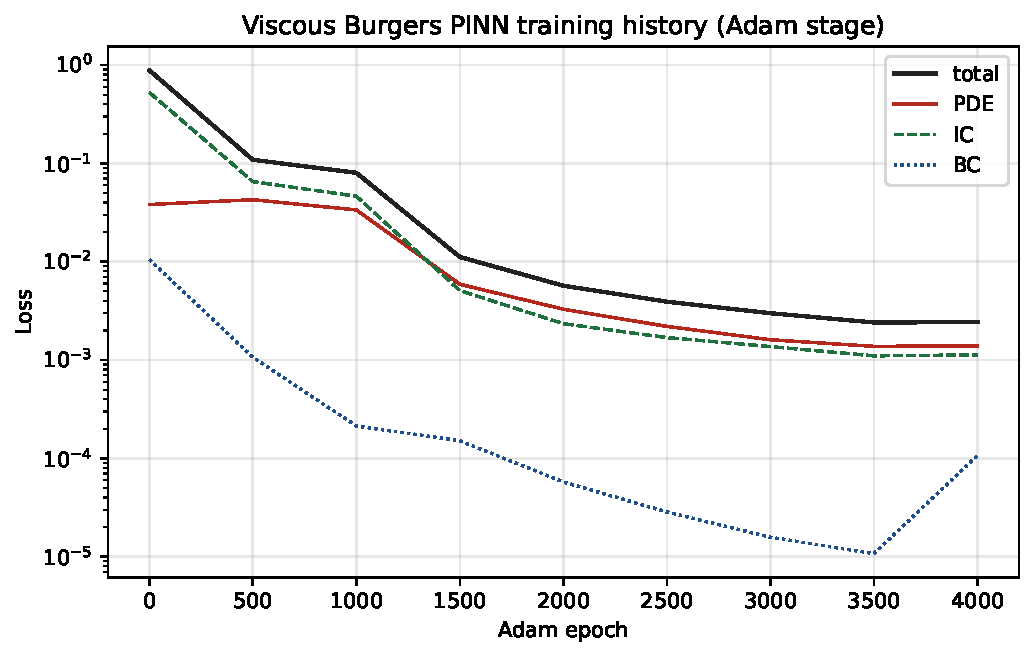
\includegraphics[width=0.7\textwidth]{fig_burgers_loss_history.pdf}
\caption{Burgers PINN training loss versus Adam epoch (logarithmic scale). The composite loss $\mathcal{L}_{\mathrm{PDE}} + \lambda_{\mathrm{IC}}\mathcal{L}_{\mathrm{IC}} + \lambda_{\mathrm{BC}}\mathcal{L}_{\mathrm{BC}}$ decreases by approximately three orders of magnitude before plateauing; the subsequent L-BFGS refinement reduces the residual by an additional one to two orders of magnitude. Plateaus or upward spikes during Adam typically indicate that the IC/BC weights need rebalancing or that the collocation point density is insufficient near the shock layer.}
\label{fig:burgers_loss_history}
\end{figure}

\begin{table}[h!]
\centering
\small
\caption{Viscous Burgers PINN snapshot accuracy. The relative $L_{2}$ error is $\|u_{\theta}(\cdot, t^{*}) - u_{\mathrm{exact}}(\cdot, t^{*})\|_{2} / \|u_{\mathrm{exact}}(\cdot, t^{*})\|_{2}$, evaluated on a uniform grid of $401$ points in $x \in [-1, 1]$. The peak pointwise error is the maximum of $|u_{\theta} - u_{\mathrm{exact}}|$ over the same grid. The largest errors concentrate inside the viscous shock layer near $x = 0$ once $t > t^{*}_{\mathrm{break}}$.}
\label{tab:burgers_errors}
\begin{tabular}{c c c c}
\toprule
$t^{*}$ & Regime & Relative $L_{2}$ error & Peak pointwise error \\
\midrule
$0.25$ & Smooth, pre-breaking               & $1.13 \times 10^{-3}$ & $2.20 \times 10^{-3}$ \\
$0.50$ & Just after breaking, layer formed  & $1.03 \times 10^{-3}$ & $1.40 \times 10^{-3}$ \\
$0.75$ & Established viscous shock layer    & $7.83 \times 10^{-4}$ & $1.79 \times 10^{-3}$ \\
\bottomrule
\end{tabular}
\end{table}

Table~\ref{tab:burgers_errors} reports the relative $L_{2}$ error and peak pointwise error at the three snapshot times. Accuracy is uniformly excellent across all three regimes, with relative $L_{2}$ error remaining below $0.12\%$ at every snapshot; the error in fact decreases slightly from $t^{*} = 0.25$ to $t^{*} = 0.75$, reflecting that the L-BFGS refinement equilibrates the residual across the full time window once the viscous layer has reached its asymptotic thickness. The numerical magnitudes are consistent and confirm that, even with a uniform collocation distribution and a single Adam-then-L-BFGS schedule, a small PINN can reproduce a viscous shock to engineering accuracy.

\subsection{Educational Insights}

The two Burgers demonstrations together expose several principles that the Fanno benchmark could not, and that transfer directly to higher-dimensional shock-resolving applications:

\begin{itemize}
    \item \textbf{From steady ODE to unsteady PDE.} The Fanno residual was a single ODE in $M$; the Burgers residual is a PDE in $(x, t)$ requiring up to three derivatives. The same workflow---autodiff residual, smooth activations, collocation sampling---scales without modification, which is the key reason PINNs are attractive for unsteady gas dynamics.
    \item \textbf{Soft versus hard conditions.} Fanno used a hard sonic anchor $\hat{F}(M) = (M-1)\,g_{\theta}(M)$. Burgers uses soft IC and BC penalties because the conditions are distributed along three manifolds rather than imposed at a point. Hard-condition transformations (for example, $u_{\theta}(x,t) = (1-x^{2})\,t\,g_{\theta}(x,t) + (1-t)\,(-\sin\pi x)$) are an effective alternative when the geometry is simple, but soft penalties remain the default for general configurations.
    \item \textbf{Discontinuities are the hard part, not nonlinearity.} The inviscid PINN tracks the rapidly steepening profile to within a few percent right up to $t = 0.28$, just below the breaking time $1/\pi$. What it cannot do is represent the post-breaking shock with a smooth network. Adding a small viscosity, as in the Raissi configuration, removes the discontinuity and recovers a problem that a $\tanh$ network can solve to sub-$0.12\%$ relative $L_{2}$ error.
    \item \textbf{Shock layers stress the residual.} Once the viscous profile breaks, the PDE residual is dominated by a thin region of width $O(\nu/\Delta u)$. With uniform sampling the optimizer eventually resolves the layer, but residual-based adaptive sampling \cite{Lu2021hPINN} accelerates this stage substantially and is recommended for stronger or moving shocks.
    \item \textbf{Two analytical references, one workflow.} The inviscid case uses the implicit characteristic equation $x = x_{0} - \sin(\pi x_{0})\,t$ inverted by Newton iteration; the viscous case uses the Cole--Hopf integral evaluated by Gauss--Hermite quadrature \cite{Cole1951, Hopf1950}. Both reference solutions are exact (modulo machine precision) and play the same role: a ground-truth anchor that makes the PINN error quantifiable before deployment to a problem without an analytical reference.
    \item \textbf{Direct bridge to the shock tube.} Burgers retains the nonlinear advection that drives shock formation in the Euler equations but drops the energy and pressure couplings. Demonstrating PINN convergence on both inviscid and viscous Burgers is therefore a necessary precursor to applying the same machinery to the Sod shock-tube problem and, beyond it, to two- or three-dimensional compressible flows.
\end{itemize}

\subsection{Section Summary}

The two Burgers demonstrations have shown that the PINN methodology developed for the Fanno ODE generalises cleanly to a time-dependent PDE in both its inviscid and viscous forms. The network architecture, the autodiff-based residual, and the optimiser protocol are essentially unchanged across the three case studies of this chapter; the modifications are confined to the input dimension, the order of the residual derivatives, the soft or hard enforcement of conditions, and an Adam-then-L-BFGS training schedule that finishes the optimisation in the high-accuracy basin.

Pedagogically, the three demonstrations form a complementary set. Fanno isolates the singular sonic point inside a steady scalar ODE; the inviscid Burgers PINN tracks a rapidly steepening profile up to but not beyond the classical breaking time of the characteristic flow; the viscous Burgers PINN, in the canonical configuration of Raissi, Perdikaris, and Karniadakis~\cite{Raissi2019PINN}, resolves a thin internal viscous layer to engineering accuracy with only the governing PDE and soft IC and BC penalties. Together, they cover the two structural difficulties---singularities of the governing equation and discontinuities of its solution---that practitioners will face when extending PINNs to the full Sod shock-tube problem and to multidimensional compressible flows.

\renewcommand{\bibname}{References}
\begin{thebibliography}{99}

% ---- Classical Gas Dynamics ----
\bibitem{Anderson1990}
J.~D.~Anderson, \textit{Modern Compressible Flow with Historical Perspective}, 2nd ed., McGraw-Hill, 1990.

\bibitem{Pontes2019}
J.~Pontes, N.~Mangiavacchi, G.~R.~Anjos, \textit{An Introduction to Compressible Flows with Applications: Quasi-One-Dimensional Approximation and General Formulation for Subsonic, Transonic and Supersonic Flows}, Springer, 2019.
\href{https://doi.org/10.1007/978-3-030-33253-2}{doi:10.1007/978-3-030-33253-2}.

\bibitem{Anderson2021}
J.~D.~Anderson, \textit{Fundamentals of Aerodynamics}, 7th ed., McGraw-Hill, 2021.

\bibitem{White2011}
F.~M.~White, \textit{Fluid Mechanics}, 7th ed., McGraw-Hill, 2011.

\bibitem{Duraisamy2019}
K.~Duraisamy, G.~Iaccarino, H.~Xiao, ``Turbulence Modeling in the Age of Data,'' \textit{Annual Review of Fluid Mechanics}, vol.~51, pp.~357--377, 2019.
\href{https://doi.org/10.1146/annurev-fluid-010518-040547}{doi:10.1146/annurev-fluid-010518-040547}.

% ---- Machine Learning Foundations ----
\bibitem{Brunton2020}
S.~L.~Brunton, J.~N.~Kutz, \textit{Data-Driven Science and Engineering: Machine Learning, Dynamical Systems, and Control}, Cambridge University Press, 2020.
\href{https://doi.org/10.1017/9781108380690}{doi:10.1017/9781108380690}.

\bibitem{Goodfellow2016}
I.~Goodfellow, Y.~Bengio, A.~Courville, \textit{Deep Learning}, MIT Press, 2016.
\url{https://www.deeplearningbook.org/}.

\bibitem{Ramachandran2017}
P.~Ramachandran, B.~Zoph, Q.~V.~Le, ``Searching for Activation Functions,'' arXiv:1710.05941, 2017.
\href{https://doi.org/10.48550/arXiv.1710.05941}{doi:10.48550/arXiv.1710.05941}.

\bibitem{Kingma2015Adam}
D.~P.~Kingma, J.~Ba, ``Adam: A Method for Stochastic Optimization,'' in \textit{Proceedings of the 3rd International Conference on Learning Representations (ICLR)}, 2015.
\href{https://doi.org/10.48550/arXiv.1412.6980}{doi:10.48550/arXiv.1412.6980}.

\bibitem{Prechelt1998}
L.~Prechelt, ``Early Stopping---But When?'' in \textit{Neural Networks: Tricks of the Trade}, Lecture Notes in Computer Science, vol.~1524, Springer, pp.~55--69, 1998.
\href{https://doi.org/10.1007/3-540-49430-8_3}{doi:10.1007/3-540-49430-8\_3}.

% ---- Physics-Informed Neural Networks (PINNs) ----
\bibitem{Raissi2019PINN}
M.~Raissi, P.~Perdikaris, G.~E.~Karniadakis, ``Physics-Informed Neural Networks: A Deep Learning Framework for Solving Forward and Inverse Problems Involving Nonlinear Partial Differential Equations,'' \textit{Journal of Computational Physics}, vol.~378, pp.~686--707, 2019.
\href{https://doi.org/10.1016/j.jcp.2018.10.045}{doi:10.1016/j.jcp.2018.10.045}.

\bibitem{Cuomo2022}
S.~Cuomo, V.~S.~di~Cola, F.~Giampaolo, G.~Rozza, M.~Raissi, F.~Piccialli, ``Scientific Machine Learning Through Physics-Informed Neural Networks: Where We Are and What's Next,'' \textit{Journal of Scientific Computing}, vol.~92, art.~88, 2022.
\href{https://doi.org/10.1007/s10915-022-01939-z}{doi:10.1007/s10915-022-01939-z}.

\bibitem{Roohi2025}
E.~Roohi, ``Deep Learning Surrogates for Gas Dynamics: A Physics-Informed Pedagogical Approach,'' arXiv:2512.09193, 2025.
\href{https://doi.org/10.48550/arXiv.2512.09193}{doi:10.48550/arXiv.2512.09193}.

\bibitem{Michaloglou2025}
A.~Michaloglou, I.~Papadimitriou, I.~Gialampoukidis, S.~Vrochidis, I.~Kompatsiaris, ``Physics-Informed Neural Networks in Materials Modeling and Design: A Review,'' \textit{Archives of Computational Methods in Engineering}, 2025.
\href{https://doi.org/10.1007/s11831-025-10448-9}{doi:10.1007/s11831-025-10448-9}.

\bibitem{Ren2025}
Z.~Ren, S.~Zhou, D.~Liu, Q.~Liu, ``Physics-Informed Neural Networks: A Review of Methodological Evolution, Theoretical Foundations, and Interdisciplinary Frontiers Toward Next-Generation Scientific Computing,'' \textit{Applied Sciences}, vol.~15, no.~14, art.~8092, 2025.
\href{https://doi.org/10.3390/app15148092}{doi:10.3390/app15148092}.

\bibitem{Urban2025}
J.~F.~Urb\'an, P.~Stefanou, J.~A.~Pons, ``Unveiling the Optimization Process of Physics-Informed Neural Networks: How Accurate and Competitive Can PINNs Be?,'' \textit{Journal of Computational Physics}, vol.~523, art.~113656, 2025.
\href{https://doi.org/10.1016/j.jcp.2024.113656}{doi:10.1016/j.jcp.2024.113656}.

\bibitem{Lu2021hPINN}
L.~Lu, R.~Pestourie, W.~Yao, Z.~Wang, F.~Verdugo, S.~G.~Johnson, ``Physics-Informed Neural Networks with Hard Constraints for Inverse Design,'' \textit{SIAM Journal on Scientific Computing}, vol.~43, no.~6, pp.~B1105--B1132, 2021.
\href{https://doi.org/10.1137/21M1397908}{doi:10.1137/21M1397908}.

\bibitem{Jagtap2020}
A.~D.~Jagtap, K.~Kawaguchi, G.~E.~Karniadakis, ``Adaptive Activation Functions Accelerate Convergence in Deep and Physics-Informed Neural Networks,'' \textit{Journal of Computational Physics}, vol.~404, art.~109136, 2020.
\href{https://doi.org/10.1016/j.jcp.2019.109136}{doi:10.1016/j.jcp.2019.109136}.

\bibitem{Kharazmi2021}
E.~Kharazmi, Z.~Zhang, G.~E.~Karniadakis, ``hp-VPINNs: Variational Physics-Informed Neural Networks with Domain Decomposition,'' \textit{Computer Methods in Applied Mechanics and Engineering}, vol.~374, art.~113547, 2021.
\href{https://doi.org/10.1016/j.cma.2020.113547}{doi:10.1016/j.cma.2020.113547}.

\bibitem{LiuNocedal1989}
D.~C.~Liu, J.~Nocedal, ``On the Limited Memory BFGS Method for Large Scale Optimization,'' \textit{Mathematical Programming}, vol.~45, no.~1--3, pp.~503--528, 1989.
\href{https://doi.org/10.1007/BF01589116}{doi:10.1007/BF01589116}.

% ---- Burgers' Equation and Shock-Wave Dynamics ----
\bibitem{Burgers1948}
J.~M.~Burgers, ``A Mathematical Model Illustrating the Theory of Turbulence,'' \textit{Advances in Applied Mechanics}, vol.~1, pp.~171--199, 1948.
\href{https://doi.org/10.1016/S0065-2156(08)70100-5}{doi:10.1016/S0065-2156(08)70100-5}.

\bibitem{Cole1951}
J.~D.~Cole, ``On a Quasi-Linear Parabolic Equation Occurring in Aerodynamics,'' \textit{Quarterly of Applied Mathematics}, vol.~9, no.~3, pp.~225--236, 1951.
\href{https://doi.org/10.1090/qam/42889}{doi:10.1090/qam/42889}.

\bibitem{Hopf1950}
E.~Hopf, ``The Partial Differential Equation $u_{t} + u u_{x} = \mu u_{xx}$,'' \textit{Communications on Pure and Applied Mathematics}, vol.~3, no.~3, pp.~201--230, 1950.
\href{https://doi.org/10.1002/cpa.3160030302}{doi:10.1002/cpa.3160030302}.

\bibitem{Whitham1974}
G.~B.~Whitham, \textit{Linear and Nonlinear Waves}, Wiley-Interscience, 1974.
\href{https://doi.org/10.1002/9781118032954}{doi:10.1002/9781118032954}.

\bibitem{LeVeque2002}
R.~J.~LeVeque, \textit{Finite Volume Methods for Hyperbolic Problems}, Cambridge University Press, 2002.
\href{https://doi.org/10.1017/CBO9780511791253}{doi:10.1017/CBO9780511791253}.

\end{thebibliography}

\end{document}
